\documentclass[10pt,fullpage]{article}
\usepackage{epsfig,longtable}
\usepackage{times}
\usepackage{latexsym}
\usepackage{fancybox,subfigure}
\usepackage[normalem]{ulem}
\usepackage{amsmath}
\usepackage{mathrsfs}
\usepackage{verbatim}
\usepackage{appendix}

\usepackage{natbib}
\usepackage{bnf}
\bibpunct{[}{]}{;}{}{,}{,}
\bibliographystyle{plainnat}
%\usepackage[numbers, square]{natbib}	% citation/references
% Different font in captions
\newcommand{\captionfonts}{\small}

\setlength{\topmargin}{-0.5in}
\usepackage{latexsym}
\setlength{\columnsep}{0.5cm}
\setlength{\oddsidemargin}{-0cm}
\setlength{\evensidemargin}{-0cm}
\setlength{\textwidth}{6.8in}
\setlength{\textheight}{8.7in}

\newcommand{\old}[1]{}
\newcommand{\match}{\stackrel{M}{=}}
\newcommand{\ncite}[1]{$^{\mbox{\tiny \citep{#1}}}$}
%\newcommand{\nncite}[1]{\citep{#1}}
\newcommand{\frags}{{\cal F}}
\newcommand{\snips}{{\cal S}}
\newcommand{\A}{{\tt A}}
\newcommand{\B}{{\tt B}}
\newcommand{\gap}{{\tt -}}
\newcommand{\ideas}{\vskip 0.6cm {\bf IDEAS:\ }}
\newcommand{\motivation}{\vskip 0.6cm {\bf MOTIVATION:\ }}
\newcommand{\mcost}[2]{#1 #2}
\newcommand{\ali}{$\mbox{ }$\hspace{0.2in}}
\newcommand{\acomment}[1]{\hspace{1in}\#{\em #1}}
\newcommand{\beqn}{\begin{equation}}
\newcommand{\eeqn}{\end{equation}}
\newcommand{\captionsize}{\footnotesize}
\newcommand{\LtoN}[1]{\parallel #1 \parallel_{2}}
\newcommand{\mecca}{HapCUT$\:$}
%%%%%%%%%%%%%% FIGURE within a box
\newenvironment{boxfig}[1]{\fbox{\begin{minipage}{\linewidth}
                        \vspace{1em}
                        \makebox[0.025\linewidth]{}
                        \begin{minipage}{0.95\linewidth}
                        #1
\end{minipage}
                        \end{minipage}}}
                                                                                                                                                                            
\def\ensuretext{\textrm}
\newcommand{\Reads}{\ensuretext{{\sc Reads}}}
\newcommand{\AlignStr}{\ensuretext{{\sc AlignStr}}}
\newcommand{\Intervals}{\ensuretext{{\sc Intervals}}}
\newcommand{\Strand}{\ensuretext{{\sc Strand}}}
\newcommand{\Partner}{\ensuretext{{\sc Partner}}}
\newcommand{\MapRel}{\ensuremath{\stackrel{M}{\Leftrightarrow}}}
\newcommand{\MST}{\ensuremath{\mathit{MST}}}
\newcommand{\dist}{\ensuremath{\mathit{dist}}}
\newcommand{\TG}[2]{\ensuremath{\mathit{#1}^{(#2)}}}
\newcommand{\CC}{\ensuremath{\mathcal{CC}}}
\newcommand{\psubs}{\stackrel{\subset}{+}}
\newcommand{\rs}{\ensuremath{\mathit{R_s}}}
\newcommand{\MEC}{\ensuremath{\mathit{MEC}}}
\newcommand{\Prob}{\ensuremath{\mbox{Pr}}}
\newcommand{\fref}[1]{\mbox{Figure~\ref{#1}}}
\newcommand{\secref}[1]{\mbox{Section~\ref{#1}}}
\newcommand{\para}[1]{\vspace{2pt}\noindent\mbox{{\bf #1:} }}
\newcommand{\slimfast}{{\sc SlimGene}}

%%%%%%%%%%%%%%%%%%%%%%%%%%%%%%%%
% GenomeQL syntax
%%%%%%%%%%%%%%%%%%%%%%%%%%%%%%%%%%%
\newcommand{\gqlSelect}{{\sc select}}
\newcommand{\gqlFrom}{{\sc from}}
\newcommand{\gqlWhere}{{\sc where}}
\newcommand{\gqlAnd}{{\sc and}}
\newcommand{\gqlAvg}{{\sc avg}}
\newcommand{\gqlMin}{{\sc min}}
\newcommand{\gqlMax}{{\sc max}}
\newcommand{\gqlIn}{{\sc in}}
\newcommand{\gqlCount}{{\sc count}}
\newcommand{\gqlIntersects}{{\sc intersect}}
\usepackage{latexsym}

%%%%%%%%%%%%%%%%%%%%%%%%%%%%%  THEOREM-LIKE ENVIRONMENTS
                                                                                                                                                                            
\newtheorem{THEOREM}{{\bf  Theorem}}
\newenvironment{theorem}{\begin{THEOREM} \hspace{-.85em}  {\bf :} }%
                        {\end{THEOREM}}
\newtheorem{LEMMA}[THEOREM]{Lemma}
\newenvironment{lemma}{\begin{LEMMA} \hspace{-.85em} {\bf :} }%
                      {\end{LEMMA}}
\newtheorem{COROLLARY}[THEOREM]{Corollary}
\newenvironment{corollary}{\begin{COROLLARY} \hspace{-.85em} {\bf :} }%
                          {\end{COROLLARY}}
\newtheorem{PROPOSITION}[THEOREM]{Proposition}
\newenvironment{proposition}{\begin{PROPOSITION} \hspace{-.85em} {\bf :} }%
                            {\end{PROPOSITION}}
\newtheorem{CLAIM}[THEOREM]{Claim}
\newenvironment{claim}{\begin{CLAIM} \hspace{-.85em} {\bf :} }%
                      {\end{CLAIM}}
\newtheorem{OBSERVATION}[THEOREM]{Observation}
\newenvironment{Observation}{\begin{OBSERVATION} \hspace{-.85em} {\bf :} }%
                      {\end{OBSERVATION}}
\newtheorem{DEFINITION}{Definition}
\newenvironment{definition}{\begin{DEFINITION} \hspace{-.85em} {\bf :} }%
                           {\end{DEFINITION}}
\newcommand{\QED}{\hfill$\clubsuit$ \vskip 0.1cm}
\newenvironment{proof}{\noindent {\bf Proof:} \hspace{.677em}}{\QED}
\newenvironment{packed_enum}{
\begin{enumerate}
  \setlength{\itemsep}{1pt}
  \setlength{\parskip}{0pt}
  \setlength{\parsep}{0pt}
}{\end{enumerate}}
\newenvironment{packed_itemize}{
\begin{itemize}
  \setlength{\itemsep}{1pt}
  \setlength{\parskip}{0pt}
  \setlength{\parsep}{0pt}
}{\end{itemize}}

% define the title
\author{Vineet Bafna, Christos Kozanitis, George Varghese\thanks{CSE, UC San Diego}}
\title{Abstractions for Genomics: Or which way to the Genomic Information Age?}



% packages
\usepackage{graphicx}
%\usepackage{subfig}

%document
\begin{document}
\maketitle


\section{Introduction}

The saying that we are a product of ``nature and nurture'' is
formalized in biology by saying that a person's phenotype (any outward
characteristic, in this article especially health) is a function of
her genotype (the DNA program inside all cells) and the environment
(all the inputs to a human including food and medicine).  For a
computer scientist, this is analogous to saying that the behavior of a
program (say what is returned by Google Search) is a function of both
the program (i.e., Google search) and input (keywords typed by user).
Unlike computers, however, the ``program'' within human beings has
been largely hidden away till the completion of the Human Genome (HG)
in 2004.  While the cost of assembling HG was 100's of millions of
dollars, recent advances~\citet{} promise to drop sequencing costs to
under \$1000 using small desktop machines. {\bf NOTE: The last sentence
makes no sense. I suppose ``sequencing'' is better term than
``assembling''. Also don't mess sequencing with processing. The
sequencing cost does not involve computational costs.}

As a consequence, medicine has traditionally been ``impersonal'' with
doctors providing treatments as a function of the symptoms and not of
the distinctive features of the patients themselves.  While some
customization is done based on crude features such as weight and race,
the ability to cheaply read the program of each human promises the
ability to practice personalized medicine --- treatments based on
symptoms and the patient's distinctive program (i.e., DNA) as shown in
Figure~\ref{fig:fig1}.  A classic example is
provided by the drug warfarin. A blood-thinner, Warfarin has had
myriad uses as rat-poison~\citet{}, to treat Eisenhower~\citet{}, and
allegedly to poison Stalin~\citet{}. It is now a widely prescribed
anti-coagulant therapy against blood clot formation. The dosage is
critical: too high, and the patient can bleed to death; too low and
the drug is not effective. Often, the right dosage is established
through multiple visits to the clinic, and regular testing. However,
recent results~\citet{} suggest that knowledge of the patient's
genetic program can help establish the right dosage. The challenge
here is to undersatnd the genetic program.

\begin{figure}[h!]
  \centering
  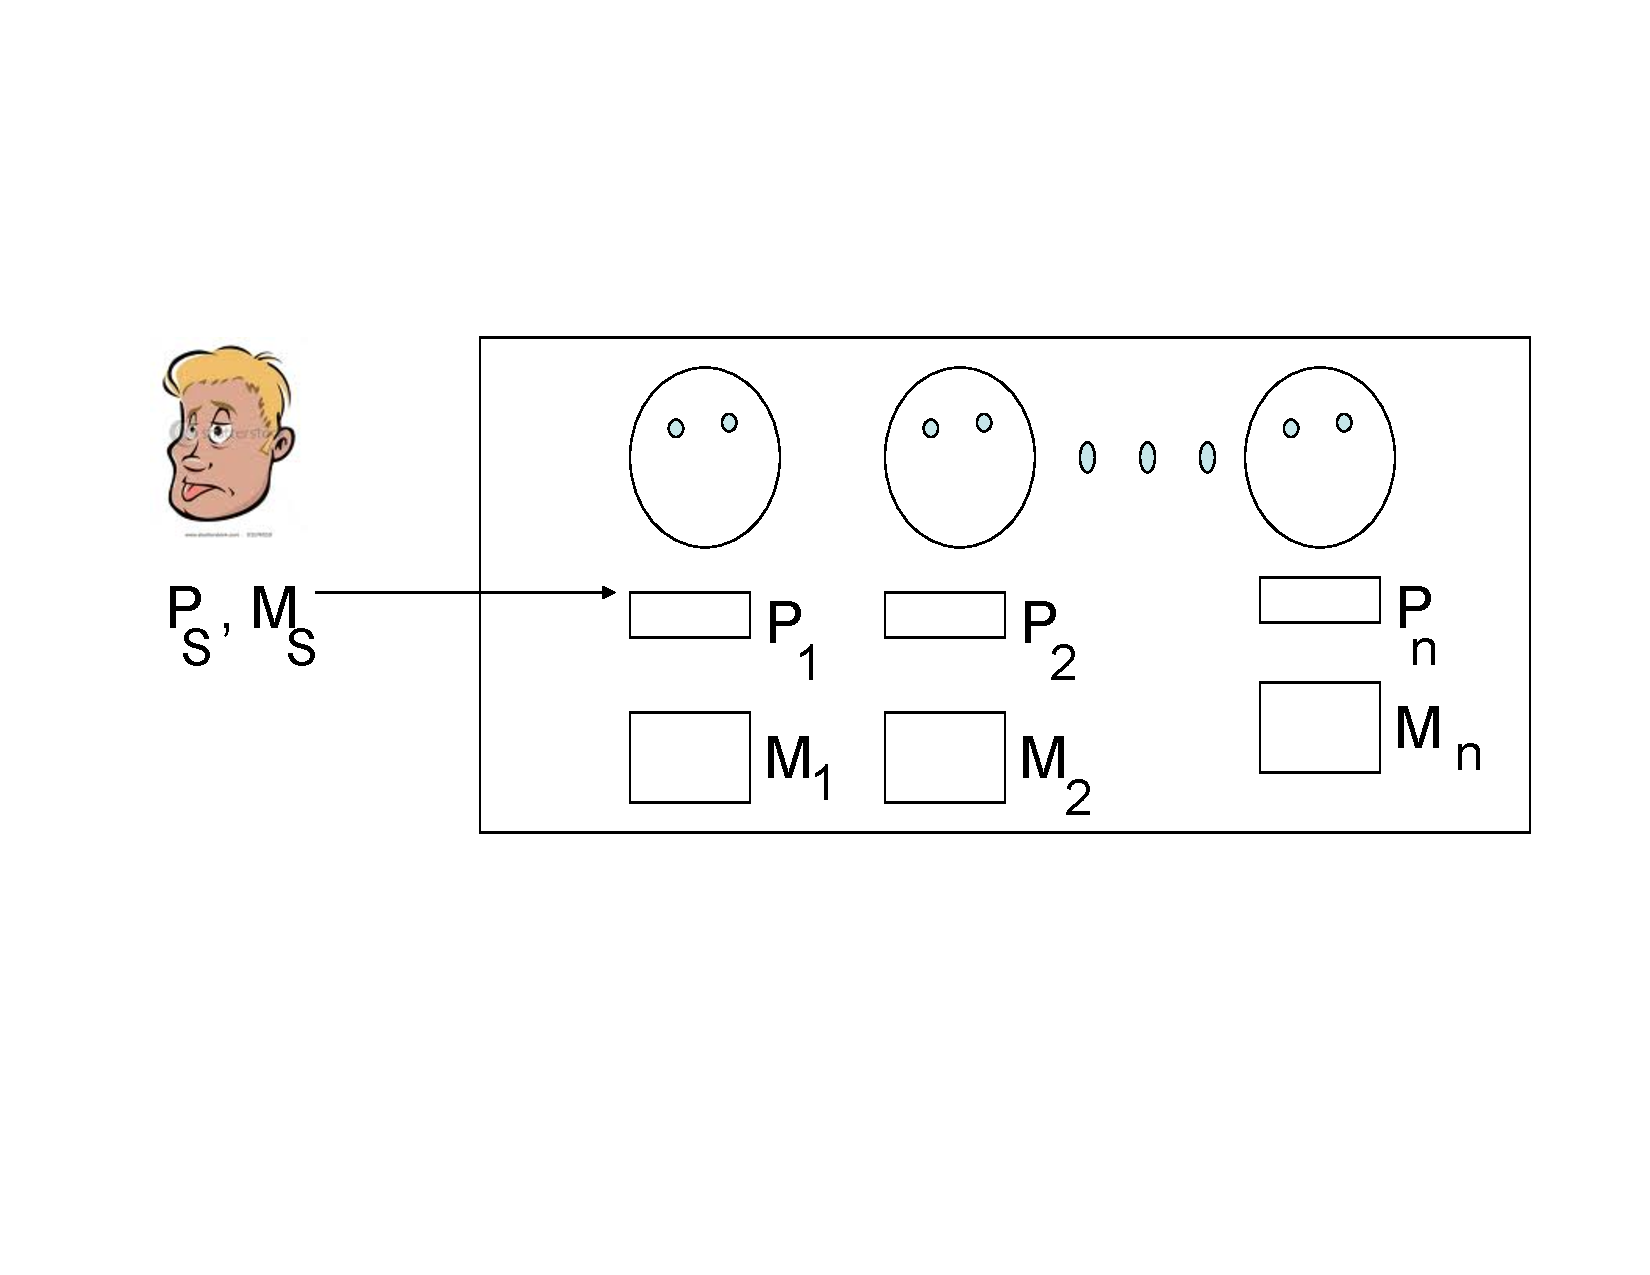
\includegraphics[trim = 25mm 70mm 20mm 50mm, clip, width=4in]{fig/personalizedmedicine.pdf}
  \caption{Personalized medicine can be seen as the task of returning the medical record and genotype of all patients `similar' to a sick patient S}
  \label{fig:fig1}
\end{figure}


This viewpoint is widely held, and a number of projects have started
with the aim of cataloging individual DNA (Figure~\ref{fig:PMD}), and
correlating variations with known phenotypes~\citep{}, using
bioinformatics and statistical genetics.  However, while the
``hardware'' costs of reading human DNA has fallen dramatically, the
software costs of analyzing the DNA has not.  (e.g. ``\$100 Genome
with a 100,000 dollar analysis''-Stanford Medicine, 2010). {\bf NOTE: is
this analysis cost a per genome cost, or the cost of the
infrastructure? Also I don't see how this paragraph connects with the
next one. Does this 100,000 dollar analysis has to do with the cost of
hiring a programmer to do the dirty work???}


\begin{figure}[h!]
  \centering
  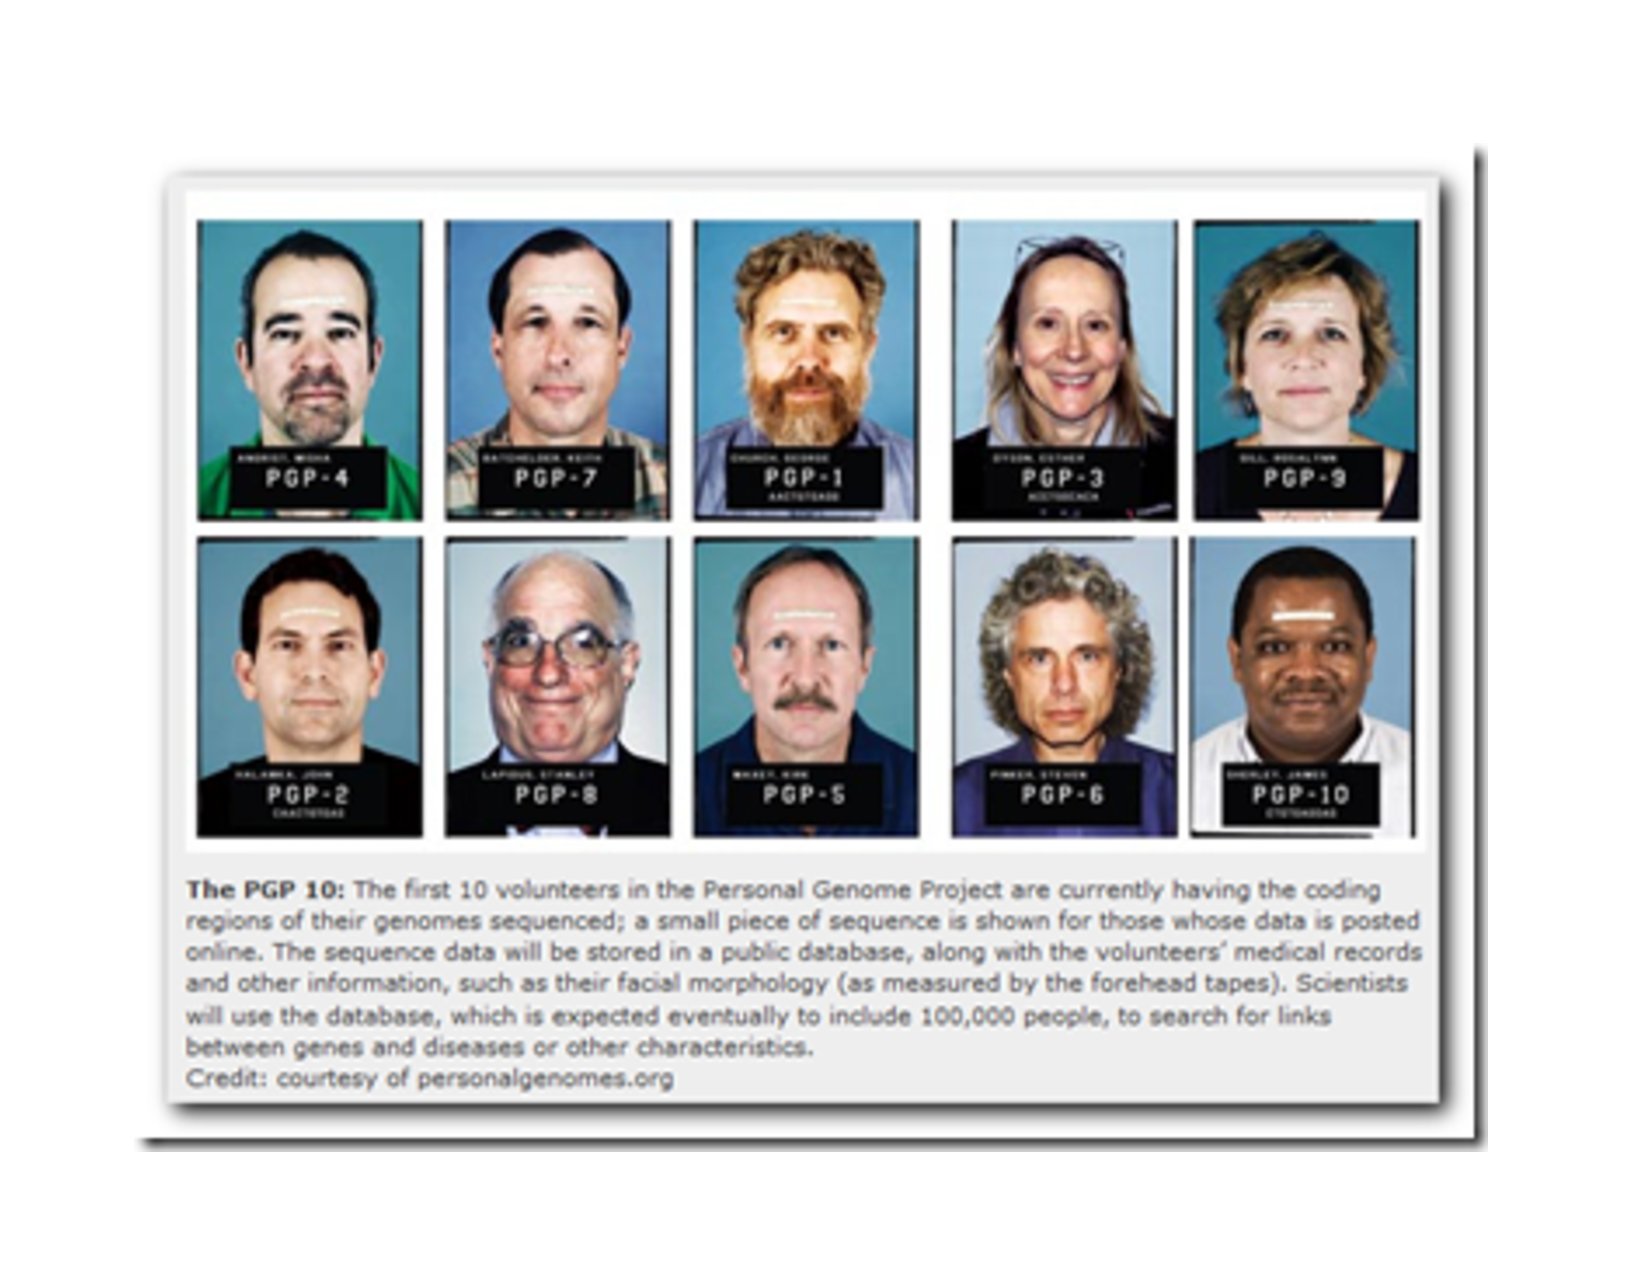
\includegraphics[trim = 0mm 20mm 0mm 20mm,clip, width=6in]{fig/PMD.pdf}
  \caption{An initial version of the Personal Medicine Database, the
    Personal Genome Project.  While the project is filling the
    database, it has not developed query abstractions. {\bf XXX we
      will need permission for this figure reproduction.}}
  \label{fig:PMD}
\end{figure}

Our central thesis in this article is that the way around this dilemma
is to invent new abstractions for genomics along with efficient
implementations thereof.  The invention of such abstractions has been
a central concern of computer system designers.  Great abstractions
such as virtual memory, time sharing, and relational data models have
vastly improved productivity and reduced software costs to keep pace
with the cheap hardware costs of VLSI.  Further, computer systems
designers have benefitted from systems thinking: making tradeoffs at
the component level for overall benefits, and leveraging technology
trends. This article is written so that computer scientists --- not
just bioinformaticians who have already contributed so much, but
computer scientists of every ilk and especially computer systems
researchers --- can engage with biologists and doctors in an essential
endeavour to improve the health of the planet.

                    
To begin the conversation, we start by describing our vision for a
vast genomic database built in layers in Section~\ref{sec:vision}.  Next, we
provide a very quick overview of the salient features of genetics in
Section~\ref{sc:genetics} using a programming metaphor so that the common questions
posed by biologists and physicians can be made accessible to computer
scientists.  In Section~\ref{} 3.0, we will provide specific ideas for new
database query abstractions --- our initial proposal for what we call
GenomeSQL -- in order to provide an example of possibly new computer
systems research that arises from genomics.  Finally, (Section~\ref{} 4.0),
we will end by outlining research directions for other aspects of
computer science --- e.g., AI, hardware design, programming languages,
and data mining --- to further this agenda.

\section{Vision}
\label{sec:vision}
A brief overview of our vision is as follows:
\begin{packed_enum}
\item By analogy with many successful computer systems, we propose
  that genomic software be layered.  For example, the Internet has
  successfully dealt with a wide variety of new link technologies
  (from dialup to wireless) and applications (from email to social
  networks) via the ``hourglass'' model using the key abstractions of
  TCP and IP (Figure~\ref{fig:abstraction}).  In the same way, we propose that Genomic
  Processing software be layered into an Instrument Layer, a
  compression layer, an evidence layer, and an inference layer that
  can separate genomic applications (e.g., cancer genomics) from
  sequencing technology.

\item We suggest that the only way to achieve such modularity is to
  forgo some possible efficiencies that could be gained by leaking
  information across layers.  For example, biological inferences can
  be sharpened by considering which sequencing technology is being
  used (Illumina versus PacBio\footnote{we shouldn't use pacbio too
    much. They might go bankrupt at anytime.}) but we suggest that
  modularity is paramount.

\item We show that the Evidence Layer can be implemented in the cloud
  while the more volatile Inference layer can be implemented in
  desktop.  We propose that while Inference methods vary considerably,
  the Evidence for inferences is fairly standard and hence propose a
  set of precise APIs between the two layers, allowing efficient
  implementation in the cloud.

\item We outline challenges for other computer science including AI
  and Learning theory researchers (to provide a standard language for
  the Inference Layer) and systems researchers (to harness other
  systems trends such as multicore and flash memory).
\end{packed_enum}
To describe our vision, we first start by an introduction to genetics
that makes it possible to describe the sample queries such a system
must support.

\begin{figure}[h!]
  \centering
  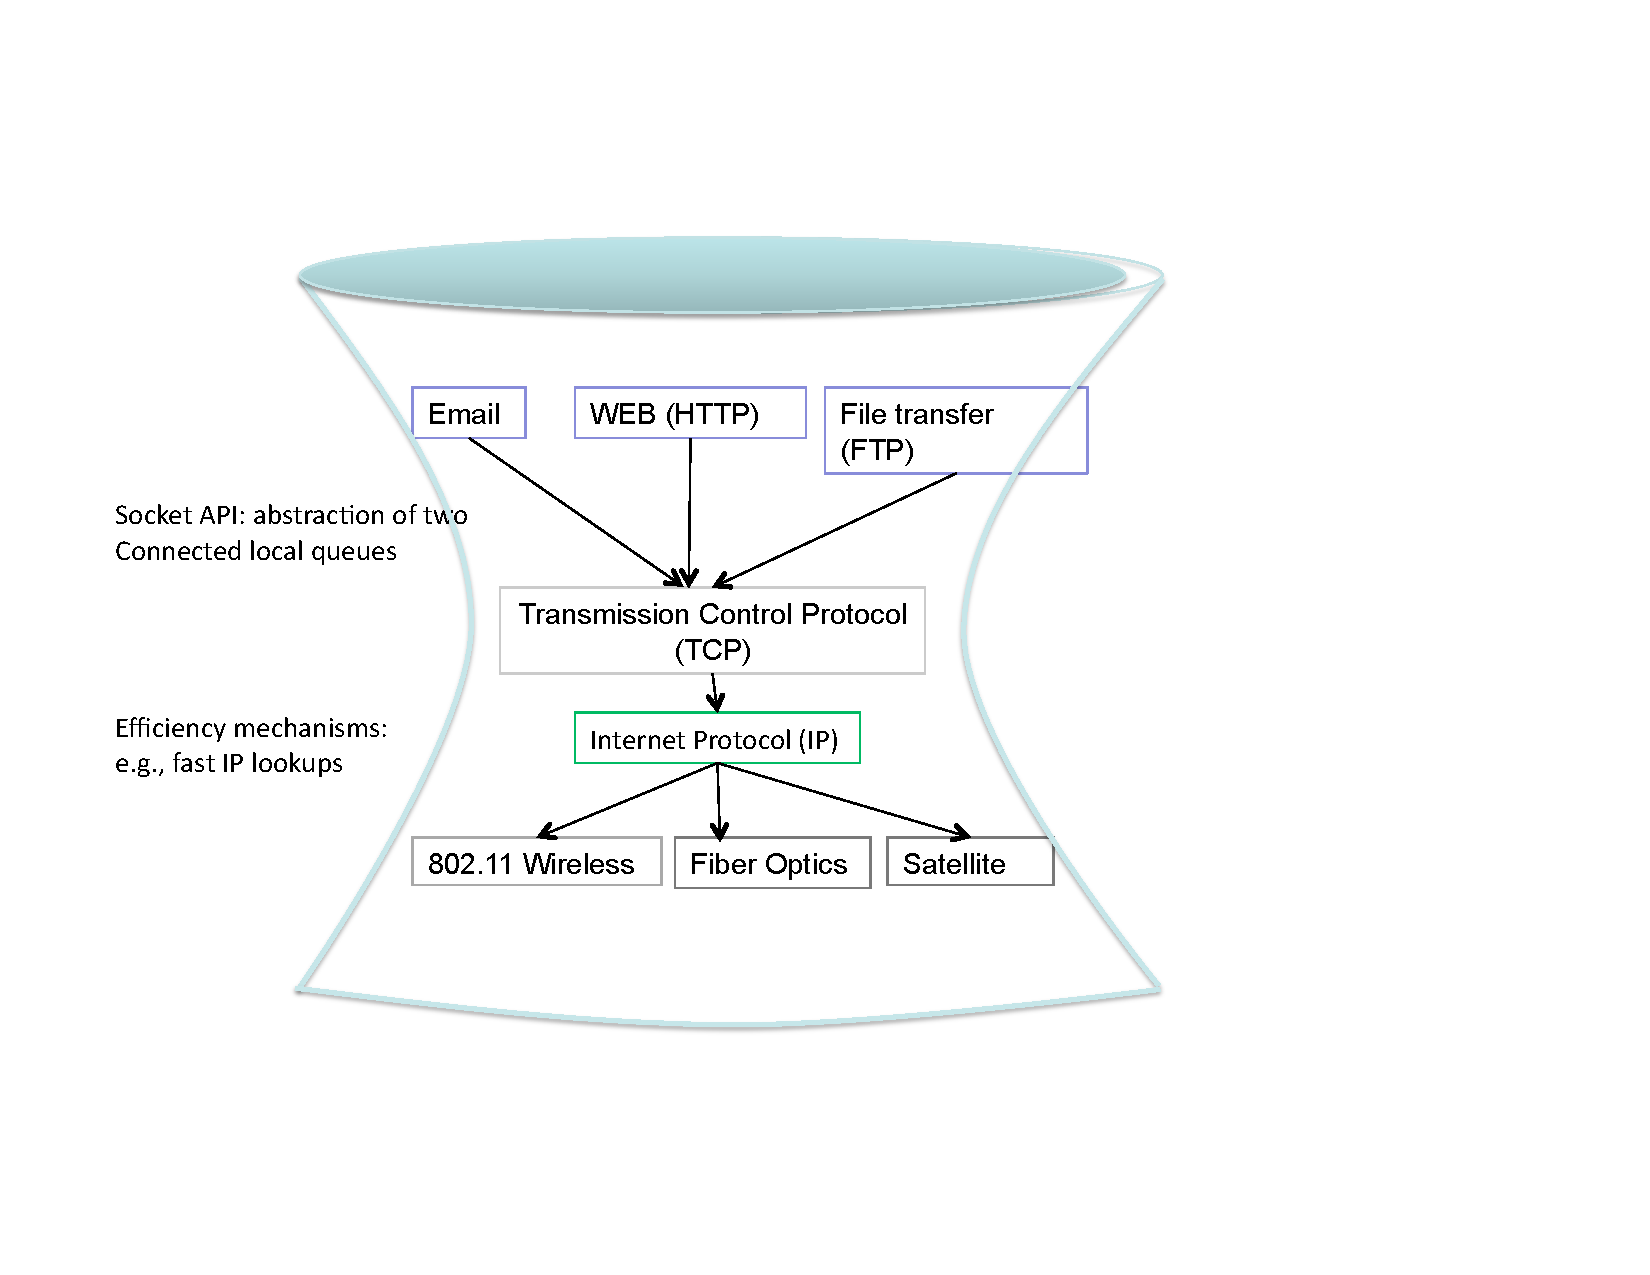
\includegraphics[trim = 0mm 40mm 60mm 10mm, clip, width=2.7in]{fig/hourglass.pdf}
  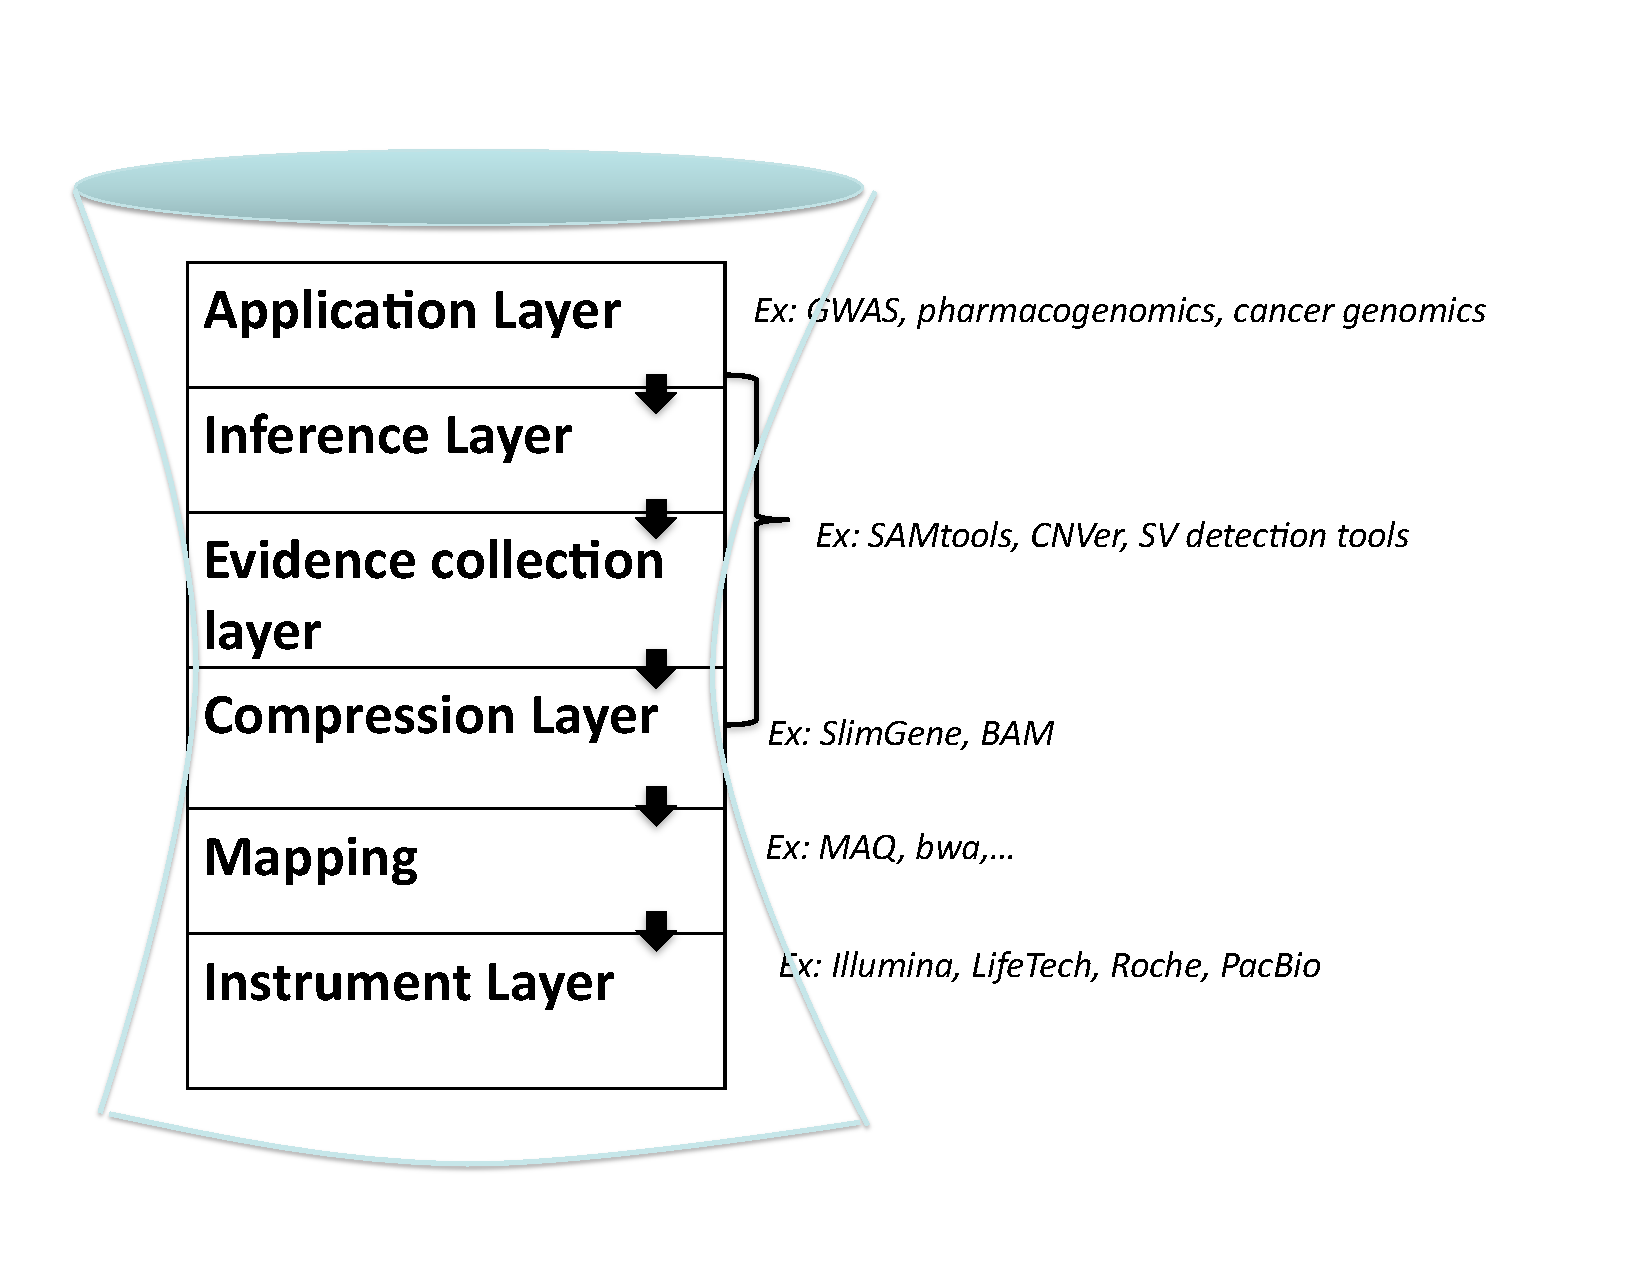
\includegraphics[trim = 0mm 10mm 0mm 20mm, clip, width=3.0in]{fig/genomicabstraction.pdf}
  \caption{Abstraction for genomics}
  \label{fig:abstraction}
\end{figure}

\section{Separating Evidence and Inference Layers}

Having understood the basics of genetics needed for understanding
important queries, we now proceed to our first idea: separating 
out the gathering of evidence required to support a query 
(deterministic, large data movement, standardized) from the inference
(probabilistic, comparitively smaller data movement, little
agreement on techiques).  The easiest way to motivate this separation
is to see how two queries are often handled: SNPs and Large Scale
Deletions.

\subsection{Calling SNPs}

Recall that SNPs are locations on the reference genome where the
patient's genome differs from the reference.   If both copies of
the patient's genome differ from the reference, the SNP is said
to be {\em homozygous} and {\em heterozygous} if only 1 copy 
differs.

Figure~\ref{Example1SNPs} shows how a SNP may be called.  Assume that
the reference has an {\em A} in a location and at least one copy
of the subject (patient) genome has a {\em C}.  How can we infer this
event from a random set of fragments (READs) of the subject genome?

Intuitively, a small number of all the READs will overlap the specified
location (roughly equal to the coverage $c$).  If there is a SNP
{\em C} do we expect all the overlapping READs to have a {\em C} in
that position.  No, there can be several confounding factors.  First,
some of the READs may have been mapped to the wrong place on the
reference; this is particularly true when the READ consists of 
repititive sequences (e.g., all C's) which are quite common.  Second,
even if the READ is mapped correctly, there could have been an error
in calling that particular base.  Third, the SNP could be heterozygous,
in which case we expect roughly half (but not exactly half because
of random variation) the overlapping READs to have a {\em C} in that
location.

Thus SNP callers often use various probabilistic based on the mapping
quality (e.g., the number of potential places in the genome a
READ can map to) of a READ, the quality score of a base call, and
the distribution of bases or alleles in the READs for that location.
Some SNP callers even use evidence based on the surrounding locations.
Some sample methods are based on P-values (what is the chance that
the evidence could have accumulated without a SNP, merely by random
chance) or by Bayesian inference (how does each READ change the 
probability that the SNP occured).   While SNP callers use various
probablistic inference technqiues, the evidence remains the same:
the set of READs overlapping the location of the SNP in question.
 
\subsection{Calling Structural Variations-- Deletions, Inversions etc}

While similar inference is done for all structural changes, 
we will take the example of a deletion of a part of the subject
genome when compared to the reference.  If both copies of
the patient's genome are deleted compared the reference, the 
deletion is said to be {\em homozygous} and {\em heterozygous} 
if only 1 copy  has the deletion.

Figure~\ref{Example2:Deletions} shows how a deletion may be called.  
Assume that the reference has the region shown in dark blue that
is deleted in at least one copy of the subject (patient) genome.
In order to detect deletions and other structural changes, we 
assume what is called Paired End mapping.  The idea is the READ
quality suffers beyond a certain length $L$ although larger 
fragments can be obtained by the shearing process.  So rather than
read the first $L$ bases of a large fragment of size $S > L$, we
can read the first $L$ and the last $L$ bases from either end of
the large fragment.  

The result is two READs that should ideally
be separated by a distance $S - L$ when mapped to the reference.
These are called {\em pairs} or {mates}.   In reality, the 
distance $S$ is not strictly controlled but has a distribution.
For example, most paired READs in Illumina processes are within
a range [1000,1500] {\bf NOTE: around 300-500} base pairs apart, with a mean of 1250(?, what
are the actual numbers).   

However, even this small variation assumes no structural changes in
the corresponding portion of the subject genome compared to the
reference.  If, as shown in Figure~\ref{Example2:Deletions} the
dark blue region is deleted, then a paired end READ of a fragment
that spans the deleted region will have the effect that the two
pairs, after mapping, now appear much further apart than the 
nominal range expected for paired ends (e.g., 1000 to 1500).   
We call these {\em discordant} READs.  Intuitively, the larger
the deletion, the larger the deviation from the norm of 1000 to 
1500.

Intuitively, a small number of all the READs will overlap the
deletion (again, roughly equal to the coverage $c$).  Once 
again we do not expect all the pairs that overlap the deleted
region to be discordant because of the usual confounding factors.  
As usual, READs may have been mapped wrongly and some may have
incorrect base calls.  Again, the deletion could be heterozygous,
in which case we expect roughly half (but not exactly half because
of random variation) the overlapping paired ends to 
be heterozygous.  Finally, there is random variation in the nominal
distribution of distance between READs.

Thus Deletion callers also use various probabilistic methods to
infer the probability of a deletion having occured.
Once again, while Deletion callers use various
probablistic inference technqiues, the evidence remains the same:
the set of discordant READs overlapping the location of the 
region in question.

Similar considerations can be used to infer inversions (one pair
READs normally and the mated pair reads backwards) and other
structural variations

\subsection{Separating Evidence from Inference}

We suggest separating out genomic query processing into two layers
because:

\begin{itemize}
\item The Evidence Layer is easier to standardize today.  As we have
seen, while there are a variety of callers, they all use the same
evidence but with a variety of heuristics and statistical techniques.
\item The separation allows Inference Layer designers to start
thinking of alternate forms of evidence to improve the confidence of
their queries.  For example, we might consider looking for 
"partially mapped" READs.  If one pair of READs overlaps the boundary
of a deletion, then that READ will match a prefix or suffix of 
the reference and the other may match perfectly.  If the mapping
shows that 1 maps correctly and the second does not, it provides
some evidence as to the location of the boundary; further a small
amount of effort can be used to decide if the non-mapped pair
has a partial match with the reference.
\item This allows the Evidence Layer to be implemented in the cloud
while the Inference Layer can be implemented either in the cloud
or in the end workstations.   We have already seen moves by Amazon
to place the 1000 genome data sets in Amazon's S3 service.  The
cloud allows rented computation on demand without the cost of
maintaining a permanent cluster by every genomics researcher.  
\end{itemize}

However, in many cases, biologists are never satisfied with a mere
call (e.g., a SNP occured in location 6000 of Chromosome 1) but 
wish to see the evidence that led to this conclusion.   Doing the
Inference Layer in the workstation allows this.  Further, if the
interface between the EL and IL is the evidence (often much smaller
than the total number of READs as we have seen), the evidence can
easily be transported across the network interactively (Mbytes
versus Gbytes).  

The standardization of the EL can lead cloud vendors to devote 
time to creating a fast and scalable EL implementation.  It is
hard to do with the IL today as it is a moving target.

In order to proceed with this idea, we need to define the interface
between the IL and the EL required to extract evidence in terms of
the relevant READs.  While we have proceeded somewhat informally,
we now continue with a formal statement of what we call an interval
calculus  that can be looked on as a form of microcode.  We will
use this "microcode" to then define many useful queries suggested
to us by equipment designers and biologists.   However, the advantage
of the calculus, is that it allows us to potentially encode
other queries as they arise in the future.  Finally, we will show
efficient indices for calculation of the queries and our 
current prototype implementations.
 

\section{Interval Calculus and genome queries}


\section{Sample Queries}

We have gathered the following queries from sequencing companies
as well as practicing biologists.  (In italics, we describe 
the corresponding translation of the query using our "programming
analogy" for computer scientists to follow more easily.  In bold
face, we show the more formal translation of the query into
interval calculus)

\begin{enumerate}

\item What is the absolute expression level of transcript X (in RPKM)? 

{\em How many times is Function(X) called in the run time Transcript normalized
by function length and the length of the execution.}

{\bf Query}: The transcript is defined by a collection of
intervals (exons) $T$. Then, if $R$ is the corpus of
reads, evidence is provided by the query\\
\noindent return $\Reads(R\MapRel T)$. 

\item What is the relative expression level of transcript X in dataset A vs. 
dataset B (fold change)? 

{\em Same as Query 1 except we compute the ratios of the expression
level in the  two data sets}

{\bf Query:} Compare evidence from $\Reads(R_A \MapRel T)$ and $\Reads(R_B \MapRel T)$.

\item Is a given regulatory pathway perturbed (up or down regulated)?  If so, how 
much? 

{\em Is there evidence for a given sequence of function calls being called
repeatedly during the execution (even though all we have is total number
of calls of each function and not the sequence of function calls)}

{\bf Query:} The pathway is defined by a set of genes, and one set of
evidence comes from looking at the change in read counts $|\Reads(R
\MapRel T)|$ of all transcripts $T$ in the pathway prior to, and post
perturbation.

\item What regulatory pathways are most perturbed and by how much? 

{\em Which sequences of function calls, especially ones implicated in past
disease execution, are likely to play a part in this diseases 
execution traces?}

{\bf Query:} Repeat previous query for all known pathways to gather the evidence.

\item What is the genotype at a specific position (SNP, indel, MNP)? 

{\em What is Line X in both Programs?} 

{\bf Query: } Define an interval $i$ by a single coordinate
(polymorphism of interest). Return $\AlignStr(R\MapRel i)$.


\item What are the diploid haplotypes (phased genotypes) across a set of linked 
loci in a dataset? 

{\em Given a set of variations of a patient's programs when compared to the 
reference, assign the variations to the patient's 
maternal and paternal programs.}

{\bf Query:} To assemble haplotypes we need a collection of reads each
of which (perhaps along with their partners) connect at least two
polymorphic sites. Let $S$ be the collection of intervals, each of
which corresponds to a single polymorphic site in the interval of
interest. Then,
\begin{packed_enum}
\item Set $R_1= \Reads(R\MapRel S)$
\item Return all $r\in R_1$ s.t. $|\Intervals (r\MapRel S)\cup \Intervals(\Partner(r)\MapRel S) |\ge 2$.
\end{packed_enum}



\item Does gene X have any deleterious mutations? (frame shift, splice site, 
stop codons, etc.)? 

{\em For a particular function, are there variations that cause
  specific bugs such as opcode misalignment, incorrect splicing of
  function code, and incorrect Return statements.}

{\bf Query}: Again, the gene is a collection of intervals (exons) $E$,
and the evidence is provided by the reads that map to the
exons. Testing for specific mutations, frame-shifts can be done by
inference on the alignments of the reads to the exons. 

Return $\AlignStr(R\MapRel E)$.

\item What loci are affected by CNVs?  What are their breakpoints?  How are they 
annotated (what genes do they involve)? 


{\em Which regions in the reference program are duplicated in the
patient's program and where are these duplications located in the 
patient's program?  Do they involve any well known functions (genes)?}

{\bf Query:} Let $I$ be a collection of intervals (for example, a
sliding window of fixed length across the genome), and $E$ be a
collection of intervals.
$I_1=\Intervals(R\MapRel I)$ s.t. $\mbox{HighCNV}(R,i,,t)$\\
Return $\cup_{i\in I_1} I:\mbox{Annot}(i,E)$.


\item Are there any other significant structural variants 
(inversion, fusion, translocation) and what functional elements 
do they cover? 



{\em Which regions in the reference program are either inverted 
(i.e., written backward), joined together, or moved to another
location in the patient's program?  Do they involve any well known 
functions (genes)?}

{\bf Inversion Discovery Query:} Let $I$ be a collection of intervals (for example, a
sliding window of fixed length across the genome), and $E$ be a
collection of intervals.  Return
$\Intervals(R\MapRel I)$ s.t. $\mbox{Inversion}(R,i,,t)$,

\item What is the methylation state of gene X (and its regulatory region)?  
How does this compare to a reference or paired sample? 

{\em Has the state of a region (function or function entry point) 
been changed to a new value?  Have any lines been commented out
(methylation can make a gene inactive analogous to commenting out
a function.) }
\end{enumerate}


\subsection{Population based queries}
We can now extend this to populations.  Assume that we 
have a large database of patients labelled with various 
phenotype
predicates $D_i$ such that $D_i(p_j)= 1$ if user $p_j$ 
satisfied predicate $D_i$.  Predicates could be, for example,
diseases ("have heart disease") or treatment outcomes 
("responded favorably to Warfarin").   We can use
standard relational queries (for example in SQL) to select
various subsets of users by combinations of predicates.
If each user $p_j$ has its DNA (or RNA) characterized by
its read set $R_j$, we can now ask questions such as:

{\bf Colloquial:} Report all intervals such that 85\% of
patients with heart disease (patients) have High Copy Number
Variation greater than threshold $r$.

{\bf Query:} Let $I$ be a collection of intervals (for example, a
sliding window of fixed length across the genome).

Let ${\cal R} = {R_j}$ be the read sets of all patients $j$
Return ${i}$ such  that $|j: HeartDisease(j)$ and
$\Intervals(R_j\MapRel i)$ and $\mbox{HighCNV}(R,i,,t)| > r$

Population queries allow us to ask for evidence about arbitrary
subsets of large groups of users based on various characteristics
of these users and doing statistical inference directly on
these large groups.  A more common approach today is for 
evidence to be returned for some variation (e.g., high copy
number or a SNP) for one user.  This evidence is then passed to an
inference layer that determines the probability or strength
of such inferences for the individual user.  The resulting
summarized variation inferences for each user (e.g., SNP in
Loc 12 with probability 0.5, Deletion in Location 1000 with
probability 0.7 etc) is then annotated with diseases and
outcomes and used to mine connections between diseases and
variations.

Instead, population queries allows the inference layer to 
bypass the determinion of individual variations for 
correlations between variations and diseases for large groups
of users.  Both are important.  For personalized medicine
and individual health, the detailed catalog of an individual's
variations are important. However, for disease correlation
studies the group variations may be more interesting.  

Further,the individual variations may have very little evidence 
(assuming even a coverage of 10, with a typical heterezygous
variation, we expect at most 5 pieces of evidence).  This
makes the strength of each individual variational inference
to be rather small.   However, if in a population of a
1000 users with a disease 850 or more had 4 length-discrepant 
regions in 
a specified interval, this is unlikely to happen by random chance
unless the deletion is correlated with the disease.  This
also implies that while individual infer must work harder to
deal with uncertainty (mapping quality, base errors) which 
can sway the balance from say 5 Reads attesting to a variation
to say 3, group inferene can be more Laissez-faire and hence
faster.  Some work on group inference for SNPs is already being
done.

Our point in what follows is not to prejudge which queries 
will be important but to build a system and a set of efficient
indices that can support both group and individual inference
and allow queries across arbitrary subsets of users and
their genetic data.

Formally, we posit a preliminary definition of a
{\em variation vector| $V_j$ for individual
$j$ is a sequence of tuples of the form $(I, c, type)$ 
where $I$ is an interval of some implicit reference such
as the human genome, $c$ is a confidence score, and 
"type" is the  type of variation (e.g., Deletion).  We 
can also extend this definition naturally to subpopulations 
(e.g., individuals with heart disease).  The task of the
Inference Layer in our model is to calculate variation vectors
for individual users (for personalized medicine) or for
subpopulations (for disease and treatment studies).   
We wish to allow queries that can support calculating 
subpopulation disease vectors either from the individual 
variation vectors of the entire population or from the
Reads of the entire population, whichever is advantageous.}

\section{Efficient Indexing}
Recall that queries have the following form:`` Given subset of reads
$R$, and subset of intervals $I$, Return {\sc Property}$(R\MapRel I)$
if {\sc Predicate}$(R\MapRel I)$''.  We say that a query is {\em
  output efficient} if its running time is a constant factor in the
size of the query output.  While we will strive for output efficiency,
for some queries we will need larger amounts of time which we will try
to quantify. It is useful to run any query in two steps:
%\begin{enumerate}
\begin{packed_enum}
\item Filter for a set of relevant reads $R$ (discard all reads that are unlikely to participate in the solution).
\item Return {\sc Property}$(R\MapRel I)$ if {\sc Predicate}$(R\MapRel I)$
\end{packed_enum}
%\end{enumerate}
We classify all queries based on two regimes: (a) Size of output
$\simeq |I|$, and (b) Size of output $<< |I|$. For a query in regime
(a), it suffices simply to do step 1 by filtering for reads that map
to interval $I$.  Define an index {\sc LocationToReads} as
follows. Sort all reads by the start point of their locations. Denote
{\sc LocationToReads}$(\ell)$ as a pointer to first read $r$ that maps
to the point-interval $l$. It is easy to see that the step 1 can be
computed by starting at the first read of the first location, and
reading off-disk sequentially. For step $2$, we simply evaluate every
read $r$ from step $1$ to see if it satisfies $r\MapRel I$. While it
is not always possible to determine a priori if the query is in regime
a or not, we can apply this approach whenever $I$ is suitable small.

However many queries involving scanning the entire genome. In these
cases $I$ (perhaps the set of all fixed size intervals throughout the
genome) is much larger than the eventual output. For efficient
implementation of these queries, we must construct special indices
that allow filtering for reads according to the predicate. Define a
{\em strength vectors} $S_P$ for a predicate $P$ as a vector of length
$G$ (the entire genome) where for any location $\ell \in I$:
\[S_P[\ell] = |\{r: r \MapRel \ell, r \in P\}|
\]
Strength vectors (with indices sorted by strength) help us efficiently
filter intervals where the variation strength is sufficiently large to
warrant inference. Thus for high and low copy numbers, we can build a
strength vector on {\sc HighCNV}. For Inversions, the predicate is
$\mbox{Inverted}(r,G)$.  For SNPs the predicate is
$\mbox{SNPDiscordant}(l,G,t)$.  For Insertions, a possible predicate
is $\mbox{HalfMapped}(r,G,t)$.

\sout{We note that if the thresholds used to determine strength are
  fixed, the strength vectors can be precomputed when Reads are added
  to the database.  It takes some time to write the Read data to the
  disk; in a small fraction of that time, the strength vector can be
  updated even as Reads come from the instrument layer. }

Strength vectors are memory intensive. To get around that, we choose a
minimum cut-off such that only intervals above the cut-off are
interesting. Define a compressed strength vector $C_{P,t}$ as a sorted
sequence of intervals $i_1, i_2, \ldots$ such that each $i_j$ is a
maximal interval satisfying $S_P[\ell] \geq t$ for all $\ell\in i_1$.
In other words, we only store the subintervals of the genome where the
strength for the predicate is sufficiently high.  Of course, if the
user changes the threshold $t$ to a lower value, the strength vectors
have to recomputed using $LocationToReads$.  \sout{But if this proviso is
accepted, even compressed strength vectors can be precomputed as Reads
are added to the database.}. Thus, we implement a query as follows:
\begin{packed_enum}
  \item Filter Intervals using $C_{P,t}$.
  \item Filter reads to get $R'=\Reads(R\MapRel C_{P,t}$.
  \item Return {\sc Property}$(R'\MapRel C_{P,t})$
\end{packed_enum}



\subsection{Population based queries}
{\bf XXX I did not change this, but we could make it more compact}. 
We now return to the population queries we introduced
earlier with the examplar query:

{\bf Query:} Let $I$ be a collection of intervals (for example, a
sliding window of fixed length across the genome).

Let ${\cal R} = {R_j}$ be the read sets of all patients $j$
Return ${i}$ such  that $|j: HeartDisease(j)$ and
$\Intervals(R_j\MapRel i)$ and $\mbox{HighCNV}(R,i,,t)| > r$

How could we efficiently compute this query without paying
a cost of $O |G| |{\ cal P}|$ where ${\cal P}$ is the subset
of patients in this query?

If we simply keep copy number strength vectors for each
patient, we will take $O |G| |{\ cal P}|$ (but this is
still less than the size of ${\cal R}$ the set of Read
sets of all patients.)  

The advantage of compressed strength vectors is that 
we can now work on large populations with much less data
not because we want to save storage (we will need to store
the Reads anyway on disk for reference) but to save time.
If the compressed strength vector is a 100 times smaller 
than the strength vector, it will be 100 times faster to
read it off disk.  This can be help speed up population 
queries.

The trick is to choose the thresholds appropriately so that
the inference layer can get a superset of what it needs,
but that is still smaller than the set of all Reads.  The
inference layer may also be interested in small regions beyond
areas of high strength.  We can do this by defining another
parameter $s$ for span and definining $CS_P(t,s)$ to be
the same intervals defined in $CS_P(t)$ except that we
augment each maximal interval $i_j$ with $s$ locations 
before and after $i_j$.

We can implement the compressed strength vectors as an interval
tree so we can now efficiently answer questions about 
predicate strength for specified annotated intervals (e.g.,
genes) in output-efficient fashion.

However, more importantly, we can now return to the examplar
query for intervals that have high copy number for patients
with heart disease.  We start with a vector of counts of length 
equal to the genome and with all counts initialied to zero.
We use a relational database to select all the "rows" 
corresponding to patients with heart disease and project out
the corresponding pointers to their compressed strength vectors.

We now traverse each compressed strength vector, incrementing the
count for each location spanned by subinterval $i$ of the
compressed strength vector for patient $j$.  We keep track
in an output queue of all locations whose counts are over some
threshold  $r$.  It should be clear that this can be generalized
to more sophisticated queries (e.g., locations in which
$X\%$ of patients have high copy number and$Y\%$ of non-patients
have low copy number).

The main idea is that we can now do population queries in time
$O V |{\ cal P}|$ where $V$ is the average length of the
number of variations in an individual in the population.  
Even if we assume variations like SNPs (millions) we have
a factor of 1000 compared to the length of the genome (billion).
But if we have variations like deletions (say 1000's) we
have larger speedups.  The reader may complain and think
that we are cheating because we precomputed the strength vectors
and so we are hiding the $O(G)$ work in precomputation.
That is indeed true but note the following.

First, if the latency can be
hidden during the still time consuming portion of data
generation that is still worthwhile.  More importantly,
after doing $O(G)$ work per user (which only takes a few msec
in our experience), we make efficient a combinatorial number of
population queries on all possible ways to slice a population
into subpopulations by combinations of atomic predicates
(e.g., diabetes and heart disease and blood pressure).  
In this case, the $O(G)$ work done once on individual $j$
can be leveraged
across all future queries that refer to individual $j$ from that
point on, including repeated queries from different users
of the database.



\section{Low leve indexing and abstractions}
This section introduces our indexing scheme and demonstrates its
capabilities by describing the implementation of a series of important
abstractions. \secref{sec:indx} describes our indexing,
\secref{sec:range} describes the range retrieval query,
\secref{sec:coverage} describes the coverage query,
\secref{sec:discordant} describes the query that finds areas that
contain multiple discordant clones and \secref{sec:haplograph}
describes creation of a haplotyping graph from a set of SNP locations.

\subsection{Indexing reads by their ranks}
\label{sec:indx}
\fref{fig:indx-descr} shows the array that indexes a file of
reads (typically a bam file). The ranking of the reads index the entries of the array. 
For example, the first entry of the table keeps the information of the
first read and so on. Each entry contains all the meta-data that
enable quick in-memory operations and also pointers for random
accessing to the read file. Thus, the index includes the location the
strand and the length of a read, its byte offset within the file and
a link to its mate entry which can be found with a pre-processing
step that groups the read-names. {\bf TODO: I don't know if the last
part makes sense. I know that it might be computationally tough to
locate mate pairs. So please let me know if we need more elaboration}.

\begin{figure}[hbt]
  \centering
  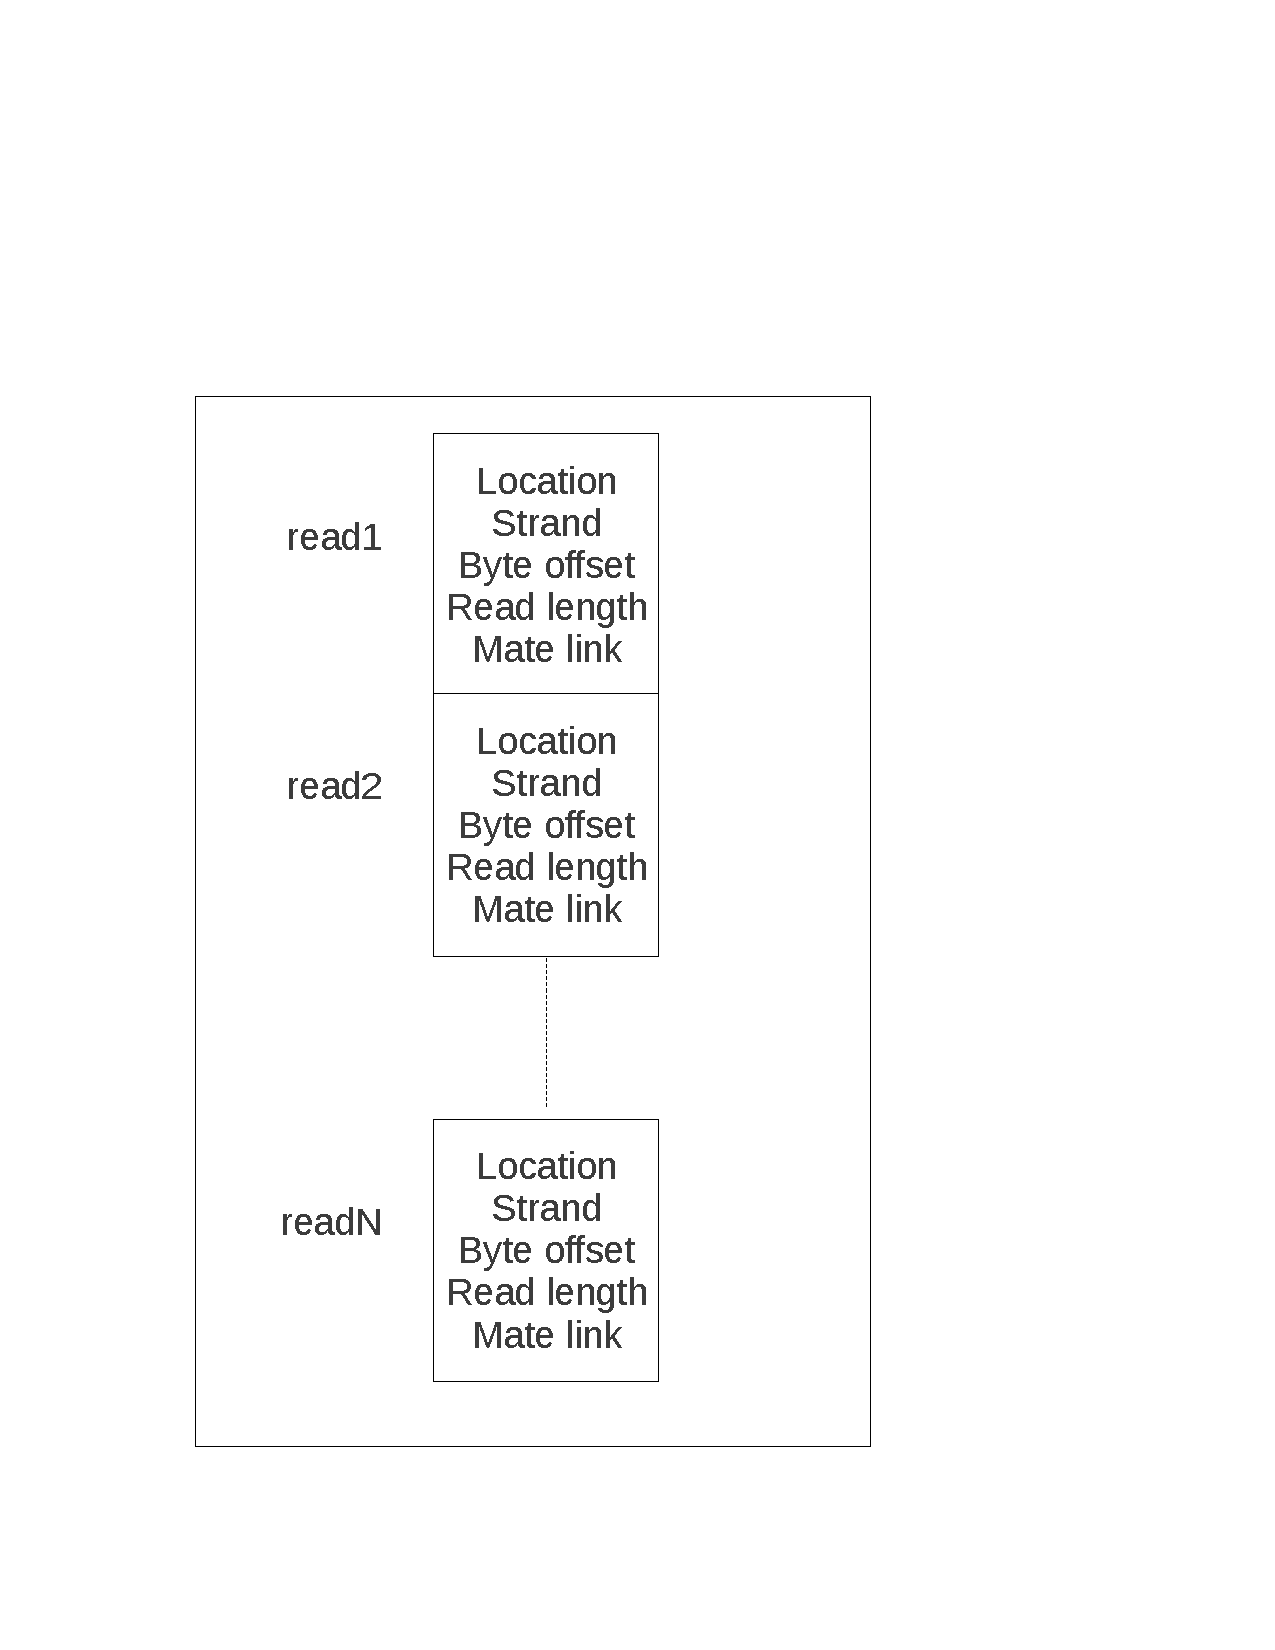
\includegraphics[trim = 30mm 30mm 60mm 40mm,
  clip,width=2in]{fig/indx_descr.pdf}
  \caption{{\footnotesize Our indexing scheme }}
  \label{fig:indx-descr}
\end{figure}


We claim that our index is small enough to fit in the main memory of
any computer. Since we use 8 bytes for the byte offset, 4 bytes for
the mapping location and the mate link, 10 bits for the read length
and 1 bit for the strand information, the size of the index of the set of
alignments of the largest chromosome (chr1) of coverage $35\times$ and
read length of $100$ is $1.5GB$. {\bf TODO in the current
implementation this is even worse. I use 2 bytes for the read length
and it seems that the indx is of size 2.3G. This is embarassing if we
compare it with the size of the bam file which is 6.1G. We might need
to compress further or go back to slimgene which gives similar
compression}.

The building of the index occurrs in a small time frame. In our
experiments, a dataset of approximately $90M$ reads from NA18507 
that map with chr1 requires $6$ minutes to create the index, while the
memory footprint of the execution does not exceed $2GB$ {\bf TODO:
verify that}.

\subsection{Searching for Ranges}
\label{sec:range}

Although the retrieval of reads that overlap with a given range is
easily implemented with the indexing scheme of Samtools, we choose to
use our existing index for such an implementation. In this way we simplify the
design by eliminating the necessity of maintaining multiple indexes.

The implementation of this query requires the knowledge of the byte
locations of the reads of the answer in the bam file. Thus we scan
sequentially the index up to the location of the entry of the first
read that overlaps with the given range. The desired byte offset is
the value of the {\em byte offset} field of the array.

Although this search on the index is more complex than the search that
samtools use, in practice the difference in time is negligible.
Obviously a sequential scan of N entries has a time complexity of O(N)
which is slowly from a lookup that samtools use which is of O(1).
However, the fetching of the actual reads from the disk eliminates the
overhead of the sequential search in the main memory.

\subsection{Retrieving Areas by Coverage}
\label{sec:coverage}
In this section we describe the implementation of the query: 
``{\em Given a constant $k$, find all regions of a chromosome which are
covered by at least $k$ reads}''. In addition we show why the
implementation with our index outperforms alternative implementations.

This query requires an auxiliary array of counters that keeps the
read counts in each position. The array has a length equal to the
length of the chromosome of interest and it is initialized to 0. Each
read increases the counters of those positions that overlap with it
and a backtracking step reports the areas of interest.

\fref{fig:coverage-example} shows the contents of the counters in an
imaginary scenario of a chromosome of length $10$ and reads of length
$2$. The value of each counter is the number of reads that overlap with 
its location. The backtracking for $k=0$ reports that areas $1$ and
$6-7$ are covered by $0$ reads. {\bf TODO: I haven't implemented the
coverage query in this way yet. This might change in the future}

\begin{figure}[hbt]
  \centering
  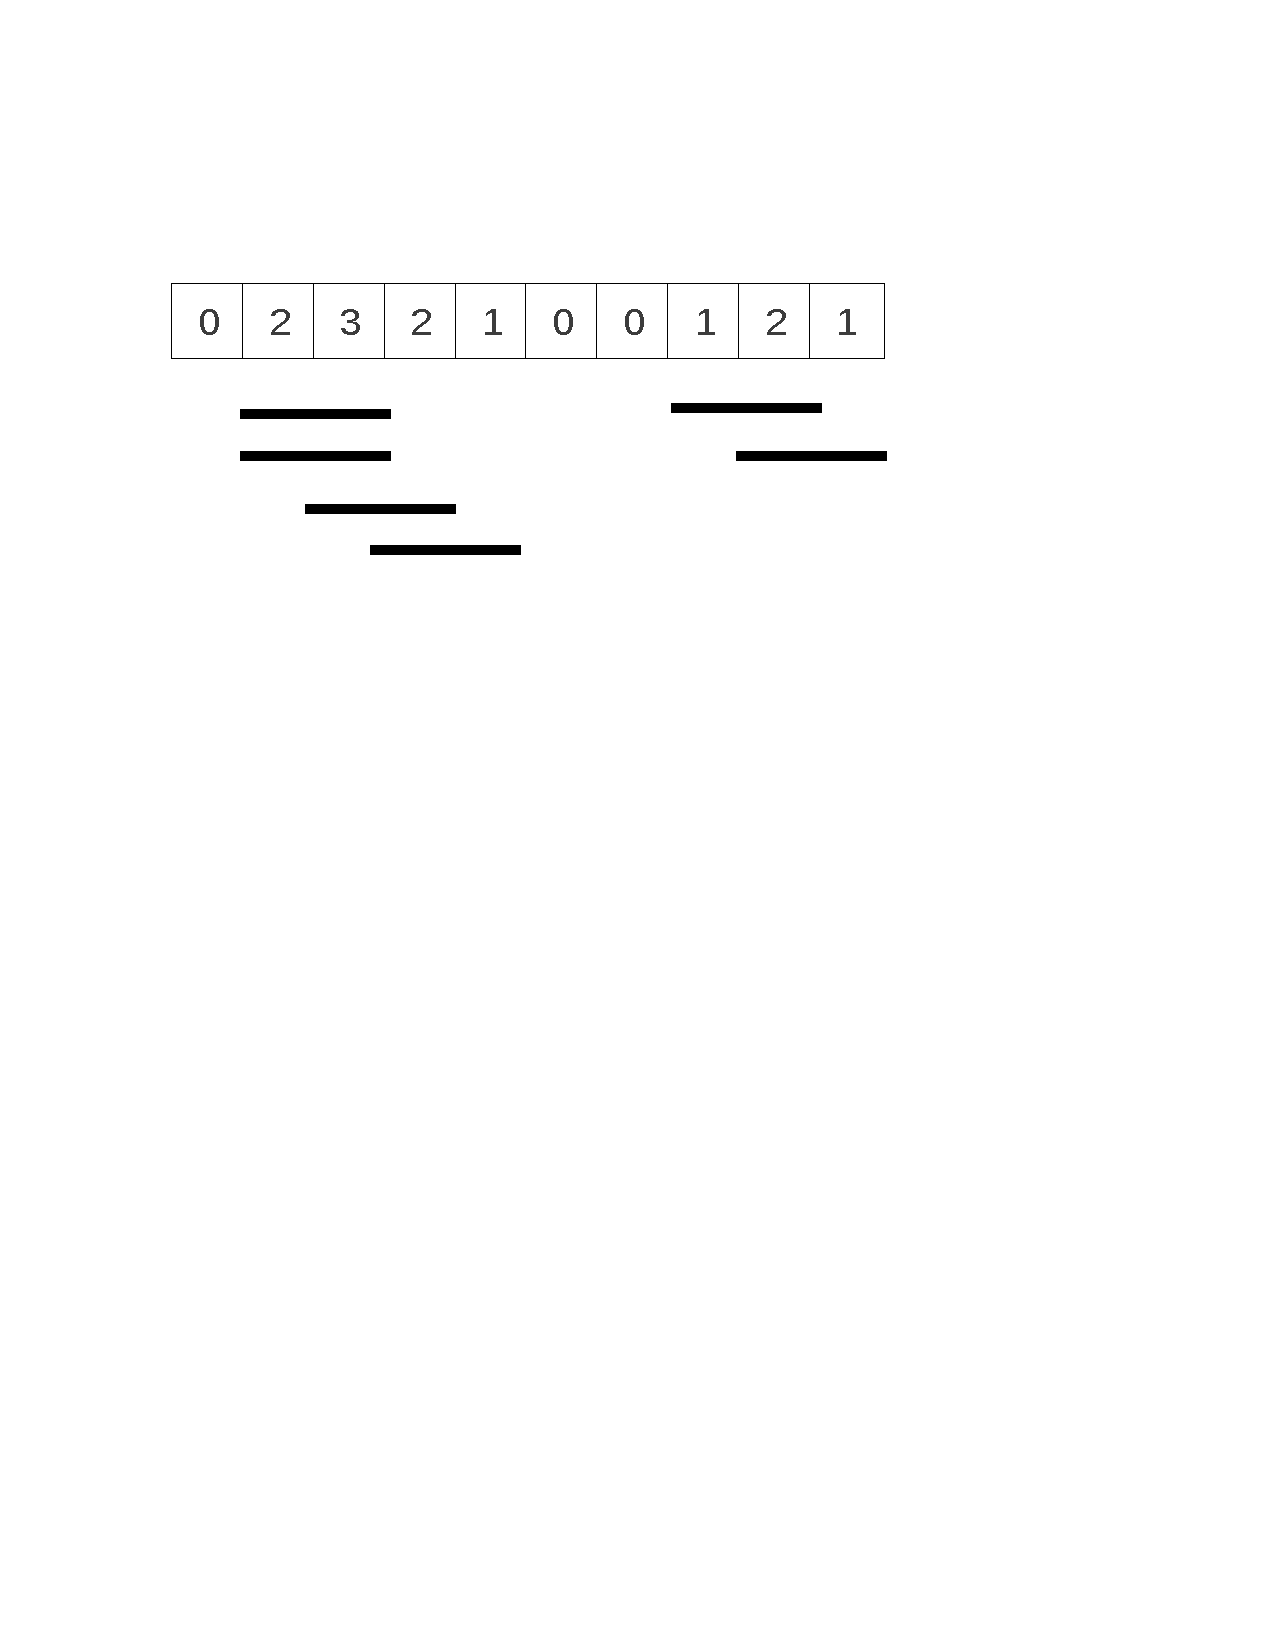
\includegraphics[trim = 15mm 185mm 60mm 40mm,clip,width=2in]{fig/coverage_example.pdf}
  \caption{{\footnotesize The auxiliary vector of counters of the
  coverage query.}}
  \label{fig:coverage-example}
\end{figure}

Of course this question can be easily answered with the pileup
function of samtools at the expense of efficiency. The pileup requires
more time to be built because it needs all the data of the input file.
Thus, the in memory manipulation of the index is more efficient. {\bf
TODO: will come back with real numbers}.

\subsection{Locating areas with discordant clones}
\label{sec:discordant}

In this section we explain how we implement the query: ``{\em Find all
regions that are covered by at least $k$ discordant clones}''. A user
can define any type of {\em discordancy} in the context of this query. 

The detection of the areas that are covered by multiple discordant
clones is proportional to the number of the discordant clones if we
model it after the balanced parenthesis problem. A left parenthesis is 
assigned for every leftmost coordinate of a discordant clone and a closing 
parenthesis is assigned for every rightmost coordinate of a discordant clone. 
Thus the area that is covered by at least $k$ discordant clones is the
area where $k$ or more parenthesis are open concurrently. Then the
solution requires a counter which increases each time a parenthesis is
open and decreases when a parenthesis closes. The regions of interest
are the areas for which the values of the counter are at least $k$.
Obviously, the number of the steps that are required by this algorithm
is equal to the number of reads that are involved in the discordant
clones.

As an example consider the discordant clones of
\fref{fig:disc-example-a}. \fref{fig:disc-example-b} shows the modeling
of the same clones with the use of parenthesis. Note that a
parenthesis opens at every position which is the starting point of a
clone and it closes at those positions that are the rightmost ends of
clones. The values of the counter appear in the bottom of this figure
and for $k=3$ the area of interest includes all positions whose value
is greater than $2$.

\begin{figure}[hbt]
  \centering
  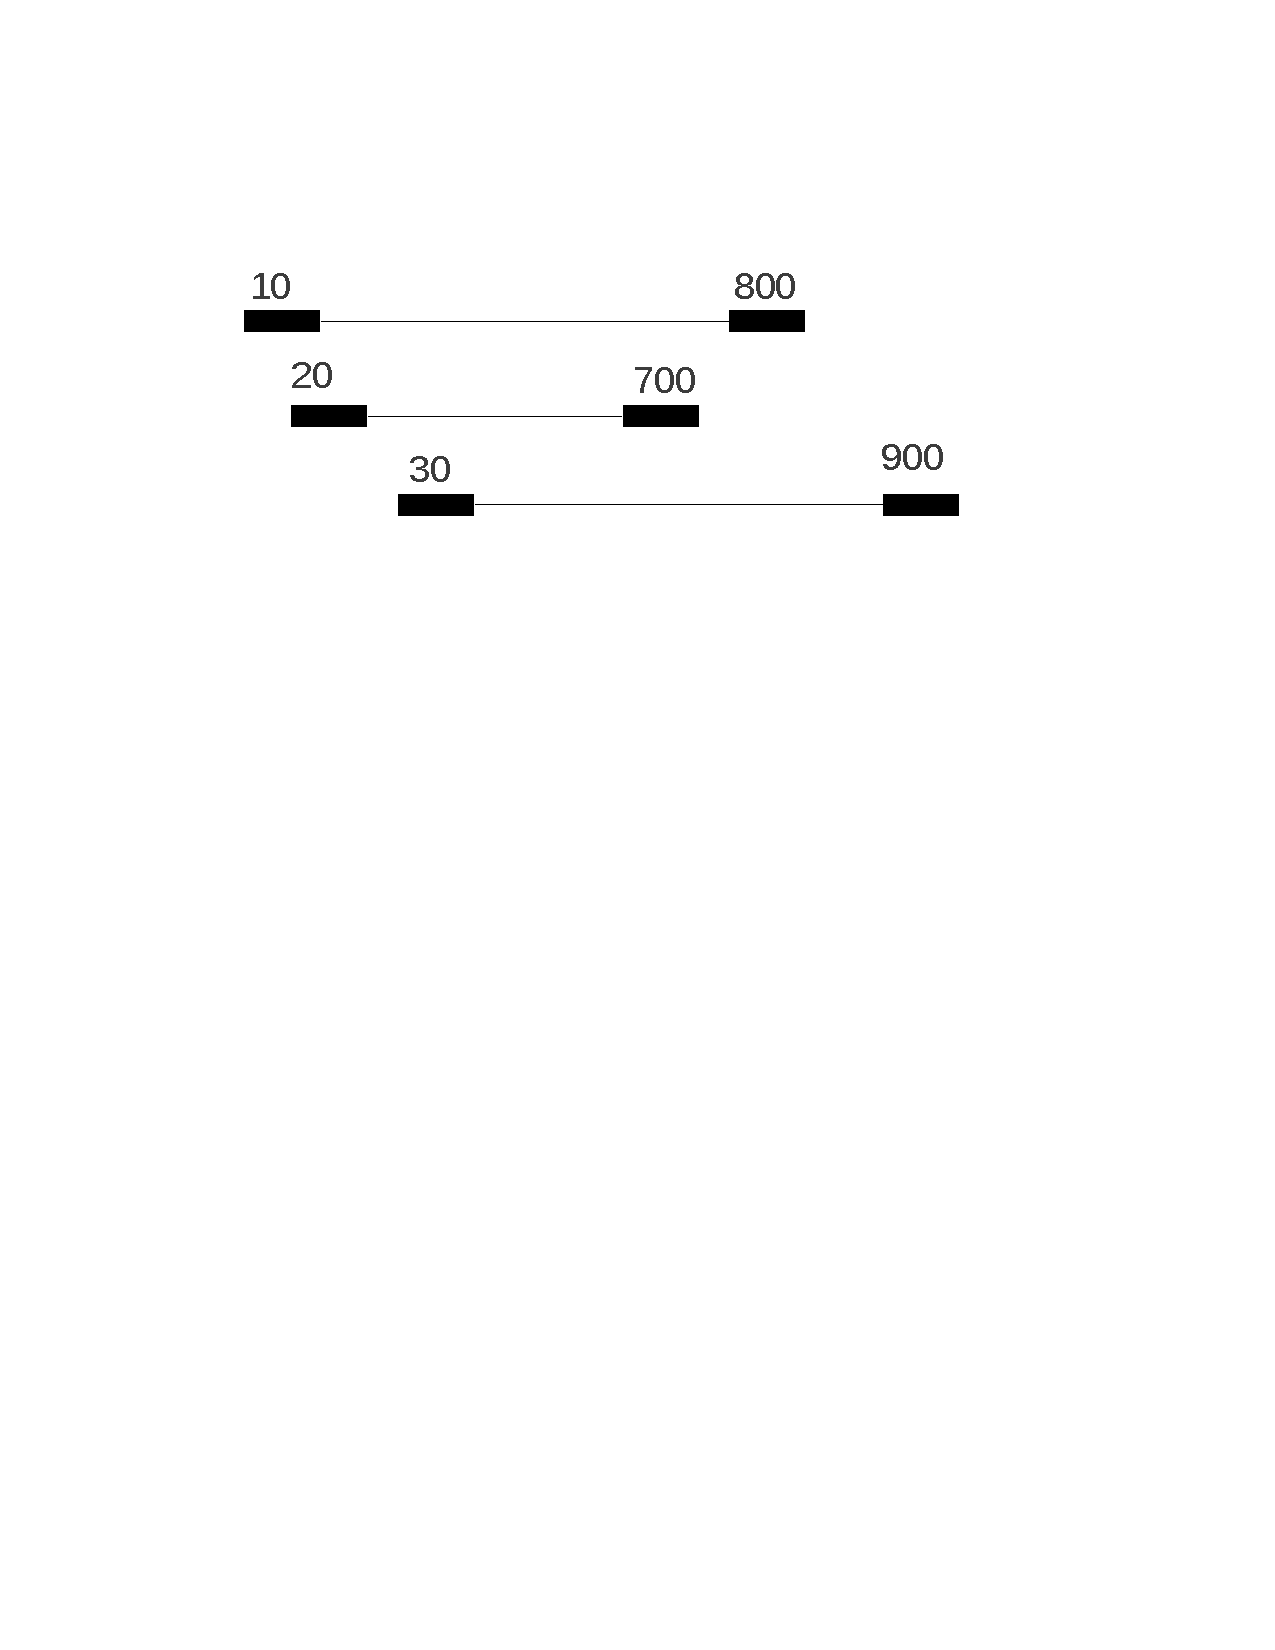
\includegraphics[trim = 30mm 190mm 55mm 40mm,
  clip,width=2in]{fig/disc_example_a.pdf}
  \caption{{\footnotesize A set of discordant clones.}}
  \label{fig:disc-example-a}
\end{figure}

\begin{figure}[hbt]
  \centering
  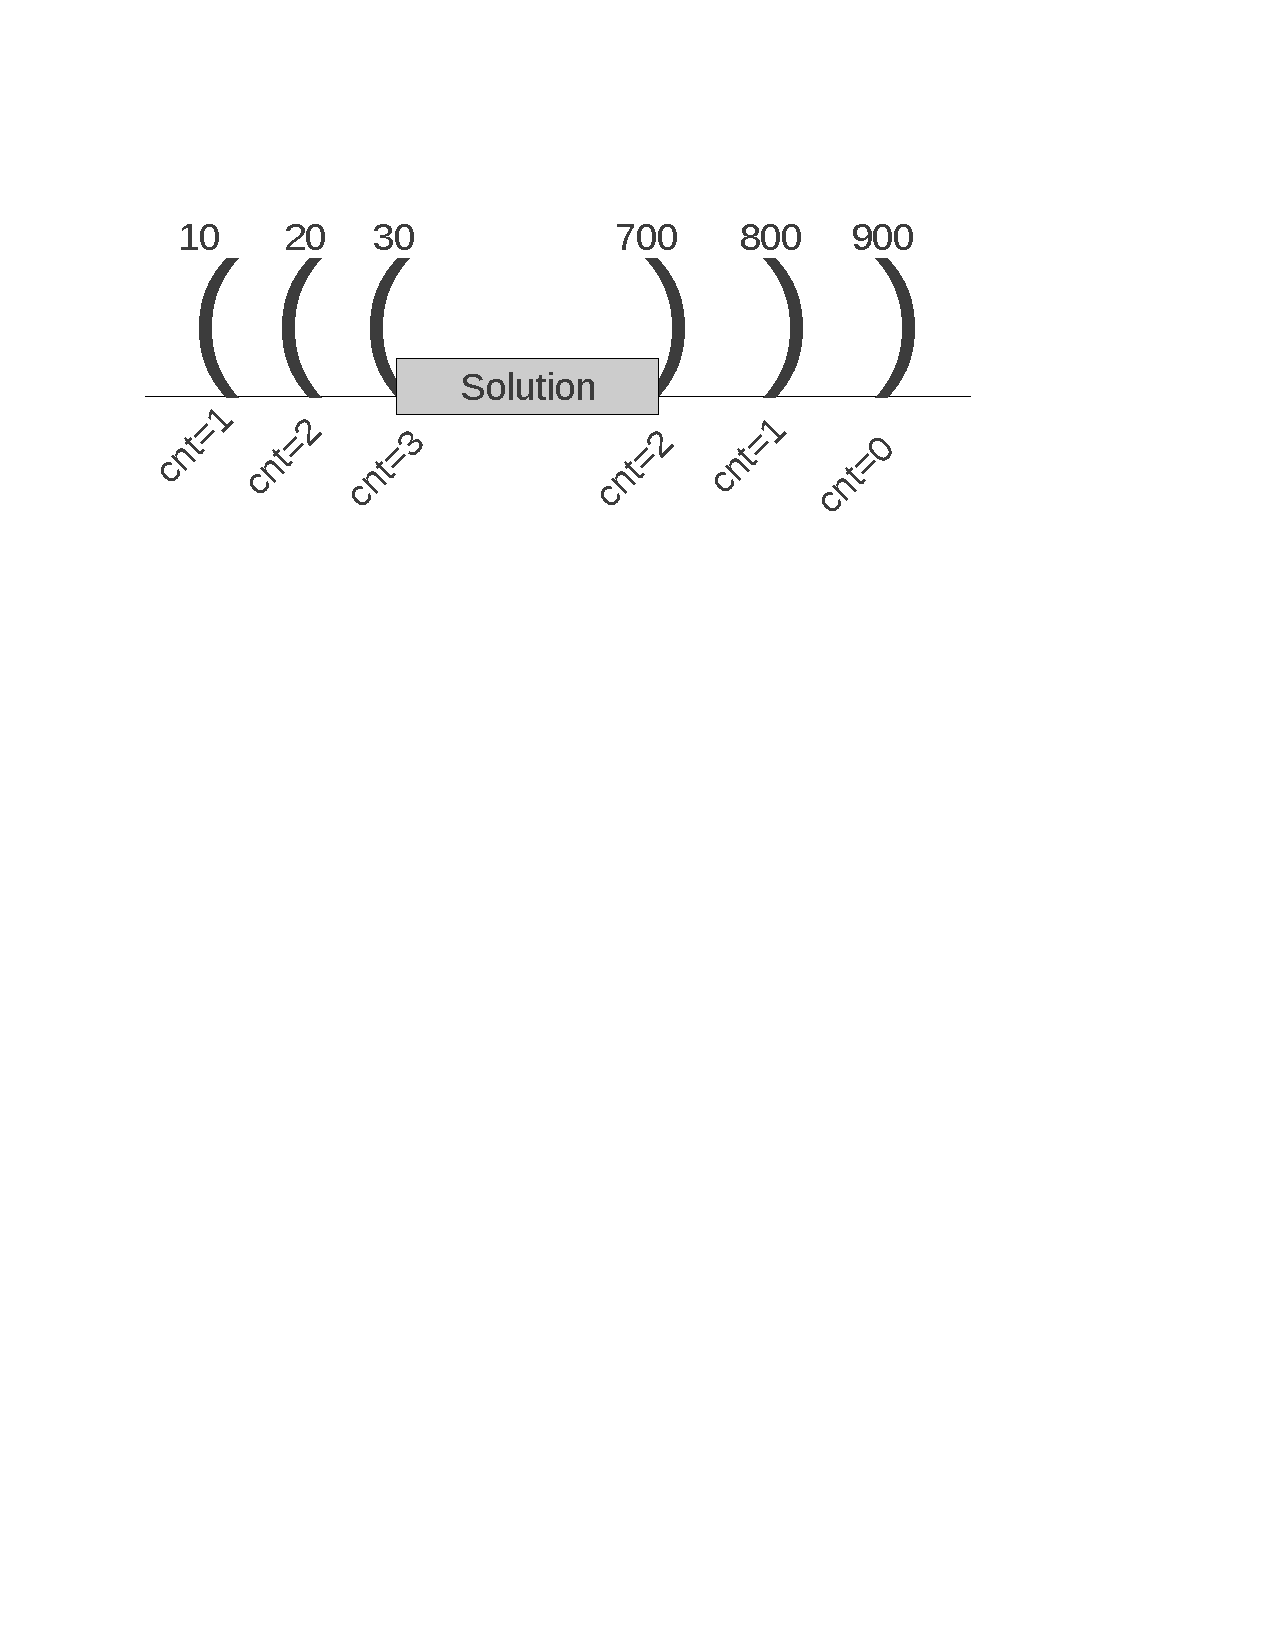
\includegraphics[trim = 25mm 190mm 55mm 30mm,
  clip,width=2in]{fig/disc_example_b.pdf}
  \caption{{\footnotesize The discordant clones are modeled
  parenthesis. The shaded area is the region which is covered by at
  least $3$ clones.}}
  \label{fig:coverage-example}
\end{figure}

\subsection{Creating a Haplotyping Graph}
\label{sec:haplograph}

In this section we describe how we implement the query:	``{\em Given a set 
of SNP loci find those pairs of reads that contain at least two of
them}''. More formally the query can be formalized as follows: {\bf
TODO: I will rewrite the following using hte algorithmic package}

\begin{itemize}
\item {\bf Input: } A set $I$ of positive integers.
\item {\bf Input: } A set $R$ of intervals of the form $\left(x_1,
x_2\right)\vee\left(x_3, x_4\right)$
\item {\bf Output: } A set $S \subset R$ such that $\forall r \in S
\exists m,n \in I and m,n \in r$.
\end{itemize}

{\bf TODO: Is there any bibliography that solves this problem with
interval trees? I would like to show that interval trees cannot do
better than our approach. If there is not such a thing available I can
give back of envelope calculations.}

An efficient implementation of this query involves a bit vector of of
the same length as the chromosome of which the elements of $I$ came
from. All positions of the bitvector that are also contained in $I$
get the value of $1$. An interval that represents a read is part of
the set $S$ if the bitvector contains $2$ or more ones in the
correspondent region.

Thus the problem is reduced to the problem of counting the number of
ones in a vector $v$. This is a well studied problem and the
number of ones of $v$ can be obtained by the number of iterations
according to which the value $v=v\&(v-1)$ is non zero. For example, if
we count the number of ones that appear in $v=5$ ($101$ in binary) in
the first iteration we have $v=5\&4=4$ and in the second iteration
$v=4\&3=0$. Thus the number of ones is $2$. 

The complexity of the algorithm is $O(|R|+|I|)$ since we count the
number of ones for all reads of $R$ and the total number of iterations
is going to be exactly equal to the number of ones of the bitvector.


\newpage
\appendix
\appendixpage
\section{Sample Queries}
\begin{minipage}[h]{0.6\linewidth}
\begin{enumerate}
\item \emph{What is the genotype at a specific position (SNP, indel, MNP)? }
  \begin{description}
   \item[EL:] Return all reads that map to location $\ell$ on chromosome $c$.
  \item[GenomeQL:] $\:\\$
    \gqlSelect\  R.all \gqlFrom\ Reads\\ \gqlWhere\ \gqlIntersects([R.chr,R.beg,R.end],[$c,\ell,\ell$]).
  \end{description}
\item\emph{Does gene $g$ have any deleterious mutations? (frame shift, splice site, stop codons, etc.)?}
  \begin{description}
  \item[EL:] Return all reads that map to the exons of gene $g$, along with their alignments. 
  \item[GenomeQL:] We have a table `Annot' of annotations, where each
    entry is an interval that represents the location of the
    annotation, an Id, and a value describing the type of
    annotation. For example, all exons of the gene would be in the
    annotation table. $\:\\$
    \gqlSelect\  R.all,I 
    \gqlFrom\ Reads, Annot\\ 
    \gqlWhere\ \gqlIntersects([R.chr,R.beg,R.end],[I.chr,I.beg,I.end])\\
    \gqlAnd\ (I.id = g).
  \end{description}
\item \emph{Which loci are affected by 'large' Structural Variations
    like deletions? }
  \begin{description}
  \item[EL:] Return all intervals, and the discordant paired-end reads
    mapping to those intervals s.t. the number of reads mapping to
    them exceeds user parameter $k$. Note that intervals are not
    specified here, and we need to create a special table with each
    entry being a location of the genome, and 
  \item[GenomeQL:]$\:$\\
    \gqlSelect\ chr, loc, R.all \\
    \gqlFrom\ Genome, Reads\\
    \gqlWhere\ (\gqlSelect\ \gqlCount(R.id)\ \gqlFrom\ Reads\\
    \ali\ali \gqlWhere\ \gqlIntersects([R.chr,R.beg,R.end],[chr,loc,loc])\\
    \ali\ali\gqlAnd\ \gqlAbs(R.end-R.beg)$>d$\\
    \ali\ali) $>k$
    \hspace{0.4in} 
  \end{description}

\item \emph{What are the diploid haplotypes (phased genotypes) across
    a set of linked loci in a dataset $D$?}
  \begin{description}
  \item[EL:] Return all pairs of loci $(\ell_1,\ell_2)\in D$ that are
    connected by a read, as well as the set of reads that connect
    them. Let Variants\_in\_D denote a table of intervals, where each
    entry is a length $1$ interval $\ell_i\in D$.
  \item[GenomeQL:] $\:$\\
    \gqlSelect\ I1.all, I2.all, R.all\\
    \gqlFrom\ Variants\_in\_D, Variants\_in\_D, Reads\\
    \gqlWhere\ (\gqlIntersects([R.chr,R.beg,R.end],[I1.chr,I1.beg,I1.end])\\
    \gqlAnd\ \gqlIntersects([R.chr,R.beg,R.end],[I2.chr,I2.beg,I2.end]))\\
  \end{description}
\item\emph{Are there any other significant structural variants
    (inversion, fusion, translocation) and what functional elements do
    they cover?}
  \begin{description}
  \item[EL:] (Deletion only; similar evidence for inversions, etc.)
    Return all intervals, and the reads mapping to those intervals
    s.t. at least $k$ distance discordant reads map to those
    intervals.
  \end{description}



\item \emph{What is the methylation state of gene X (and its regulatory region)?  
How does this compare to a reference or paired sample? }

\item \emph{What is the absolute expression level of transcript X (in RPKM)? }

\item \emph{What is the relative expression level of transcript X in dataset A vs. 
dataset B (fold change)? }

\item \emph{Is a given regulatory pathway perturbed (up or down regulated)?  If so, how 
much? }

\item \emph{What regulatory pathways are most perturbed and by how much? }


\end{enumerate}
\end{minipage}

\section{DEPRECATED: Previous notation for queries}
We are given a collection of reads $R$, and allow that normal set
operations $\cup$, $\cap$, and $|\cdot|$ (cardinality) defined on
subsets of reads. Multiple reads can come from the same physical
clone. Define {\sc Partner}(r) as set of reads that belong to the same
clone as $r$.  For the genome, we define an interval $i$ by the
chromosome and the begin and end coordinates. 

Set operations on intervals are based on an interval calculus. For
intervals $i_1,i_2$, define $i_1\cap i_2$ to be the maximum interval
common to $i_1,i_2$. Similarly, define $i_1\cup i_2$ as the minimal
interval(s) $i$ containing both $i_1,i_2$. If the intervals do not
overlap, $i_1\cap i_2=\epsilon$, and $i_1\cup i_2 = \{i_1,i_2\}$. The
definition is extended to sets as
\[I_1\cap I_2 = \{ i_1 \cap i_2: i_1\in I_1, i_2\in I_2 \}
\]
\[I_1\cup I_2 = \{ i_1 \cup i_2: i_1\in I_1, i_2\in I_2 \}
\]
Intervals can also be compared by distance. Let $\parallel
i_1-i_2\parallel$ denote the distance between the end points of the
two intervals. We set $\parallel i_1-i_2\parallel=0$ if the two
intervals overlap, {\bf I don't get this} and $\parallel i_1-i_2\parallel=\infty$ if they
come from different chromosomes. For sets, 
\[
\parallel I_1-I_2 \parallel= \min_{i_1\in I_1, i_2\in I_2} \parallel i_1-i_2 \parallel
\]


Define a binary relation $\MapRel$ on $R\times I$. The relation
$\MapRel$ is an abstraction of a mapping algorithm $M$ that maps reads
to the genome. For any read $r$, interval $i$, $r\MapRel i$ ($r$
\emph{mapsto} $i$) if and only if, the mapping of $r$ to the genome
intersects with interval $i$. Denote
\[ R\MapRel I = \{ (r,i)\in R\times I \mbox{ s.t. } r\MapRel i\}
\]


The mapping has many parameters.  For example, most mappers allow
some number of substitution, insertion or deletion errors.  The
mapper looks for the best position in $I$ that matches each 
read in $R$ with the smallest number of errors.  In the face
of deletions and insertions, most mappers will also return an
"alignment string" that describes how best the mapper aligned
the input(the READ) to the reference (interval $I$).   Many
mappers will also return alternate mappings; this is crucial
because many genomes have repetitive portions that can lead to
aliasing.  While we defined "maps to" as a relation to allow for
multiple mappings, it is easiest to initially think of "maps to" as
a function.    Finally, there are many other parameters of
READs (e.g., a vector of quality scores for each position)
and the mapping itself (e.g., a confidence score for the
mapping quality, the DNA strand to which it is mapped, etc.)


We compute many \emph{properties} on the relation; properties
are functions on the mapping relation that return any desired
parameter of the relation.  
We also define \emph{predicates}, which are boolean functions on 
the mapping relation. Finally, a
\emph{query} is a statement of the form ``Return {\sc
  Property}$(R\MapRel I)$ if {\sc Predicate}$(R\MapRel I)$''.

\subsection{Properties}
Recall that the mapping is computed by aligning (along with errors) a
read to a genomic interval. Thus, properties of interest include the
mapping coordinates, the alignment string (XXX to be defined). A
typical set of useful properties is the following:
\begin{itemize}
\item {\sc Reads}$(R\MapRel I)$: subset of reads in $R$ that map to some interval in $I$.
\item {\sc Intervals}$(R\MapRel G)$: intervals formed by mapping coordinates of $R$.
\item {\sc Intervals}$(R\MapRel I)$: {\sc Intervals}$(R\MapRel G)\cap I$.
\item {\sc AlignStr}$(R\MapRel I)$: alignment string for each 
read in {\sc Reads}(R\MapRel I).  (while there are many possible
ways to represent alignment, a simple candidate is a vector
of characters of length equal to the Read, where each character 
is either "Identical", "Insertion", or "Deletion").
\item {\sc Strand}$(R\MapRel I)$: strand for each read in {\sc Reads}(R\MapRel I).
\end{itemize}

\subsection{Predicates}

The following are useful predicates we will use as "macros"
in the sequel.

\begin{itemize}

\item
$\mbox{Mismatch}(r,l, i)$ is said to be true if when 
Read $r$ is mapped to interval $i$, position $l \in i$ 
does not match the corresponding position in $r$ or
corresponds to a deletion in $r$.  (We will use this
predicate to signal intervals where there are SNPs)

\item 

$\mbox{HighCNV}(R,i,t):|Coverage(i, R)| \ge t$
(Interval $i$ is said to High Copy Number
if the number of {\sc Reads} that map to interval $i$ is
more than some threshold $t$).

\item $\mbox{LowCNV}(R,i,t): Coverage(i, R)| \leq t$

(the Low Copy Number predicate is defined analogously)

\item $\mbox{Annot}(E,I): E\cap I\ne \epsilon$, where $E$ is a subset
  of intervals representing an annotation. (For example, 
$E$ could represent the coordinates of exons on some gene.  This
is a useful predicate to focus the query on some specified 
set of intervals with biological signifiance).

\item $\mbox{LengthDiscordant}(r,G,t): \parallel \Intervals(r\MapRel G)-\Intervals(\Partner(r)\MapRel G)\parallel>t$
(a read $r$ is Length Discordant if the distance
between the read and its partner is more than threshold $t$).

\item $\mbox{Inverted}(r,G): \Strand(r\MapRel G) \ne \Strand (\Partner(r)\MapRel G)$
(a read $r$ is considered inverted if $r$ is mapped to
a different strand from its partner, which implies that the
read and its partner are mapped in reverse directions).



\item $\mbox{SNPDiscordant}(l,G,t): |r: (r\MapRel l)$ and
$Mistmatch (r, l, G)| > t$ 

(a single location $l$ is considered to be SNP discordant if 
for there are at least $t$ Reads that map to that location, 
such that alignment string for the Read shows a difference 
between the value in that location and that of the reference)

\item $\mbox{HalfMapped}(r,G,t)$: (a read $r$ is considered 
half mapped if $r$ is mapped while its partner is not mapped;
this could be a sign of an insertion)

\item $\mbox{Deletion}(R,i,t_1, t_2):|r: LengthDiscordant(r,G,t_1)
and (r\MapRel i)|\ge t_2$
(Interval $i$ may have been deleted 
if the number of discordant {\sc Reads} that map to interval $i$ 
is more than some threshold).

\item $\mbox{Inversion}(R,i,t):|r: Inverted(r,G)
and (r\MapRel i)|\ge t$
(Interval $i$ may have been inverted
if the number of inverted{\sc Reads} that map to interval $i$ 
is more than some threshold).

\end{itemize} 





\newpage

\section{Genetics for Computer Scientists}
\label{sec:genetics}
We start by describing the structure of the DNA program as two
interacting modularized programs in Sec 1.1.; we then show how
heredity and mating can be described as program composition in Sec
1.2; we show how the program runs to produce proteins (microcode) and
also higher level functions (macrocode) in Sec 1.3; we end by
describing models for program analysis tools such as sequencing and
microarrays.  Even this limited introduction to genetics will motivate
the specific database questions we pose in Sec 2.0.

\subsection{Program Structure --- Homologous Chromosomes and Genes}
\label{sec:genes}
Many important queries to genetic data are about parts of the program
such as genes: thus it is crucial to have a simple model of program
structure.  All living creatures including human beings consist of
cells; each cell can be considered to be a computer running a program.
Humans are diploid --- a surprising fact is that there are two
programs controlling each cell, one inherited from the father and one
from the mother.

Further, as shown in Fig.~\ref{fig:chromosomes}, each program is
broken up into $23$ modules called chromosomes and within each
chomosome are sparsely scattered, small functional blocks called
genes.  The module pairs from the father and mother are called
homologous chromosomes and each human has a pair of genes, one
inherited from each parent.  Each program uses a 4-character alphabet
of bases (A,C,G,T) and is around 3 billion bases long.  (There is
further structure that can be safely ignored till we talk about
inversions --- each program is really stored as two redundant copies
called strands, and the strands are stored in 3-space using the
celebrated double helix structure discovered by Crick-Watson.)



\begin{figure}[h!]
  \centering
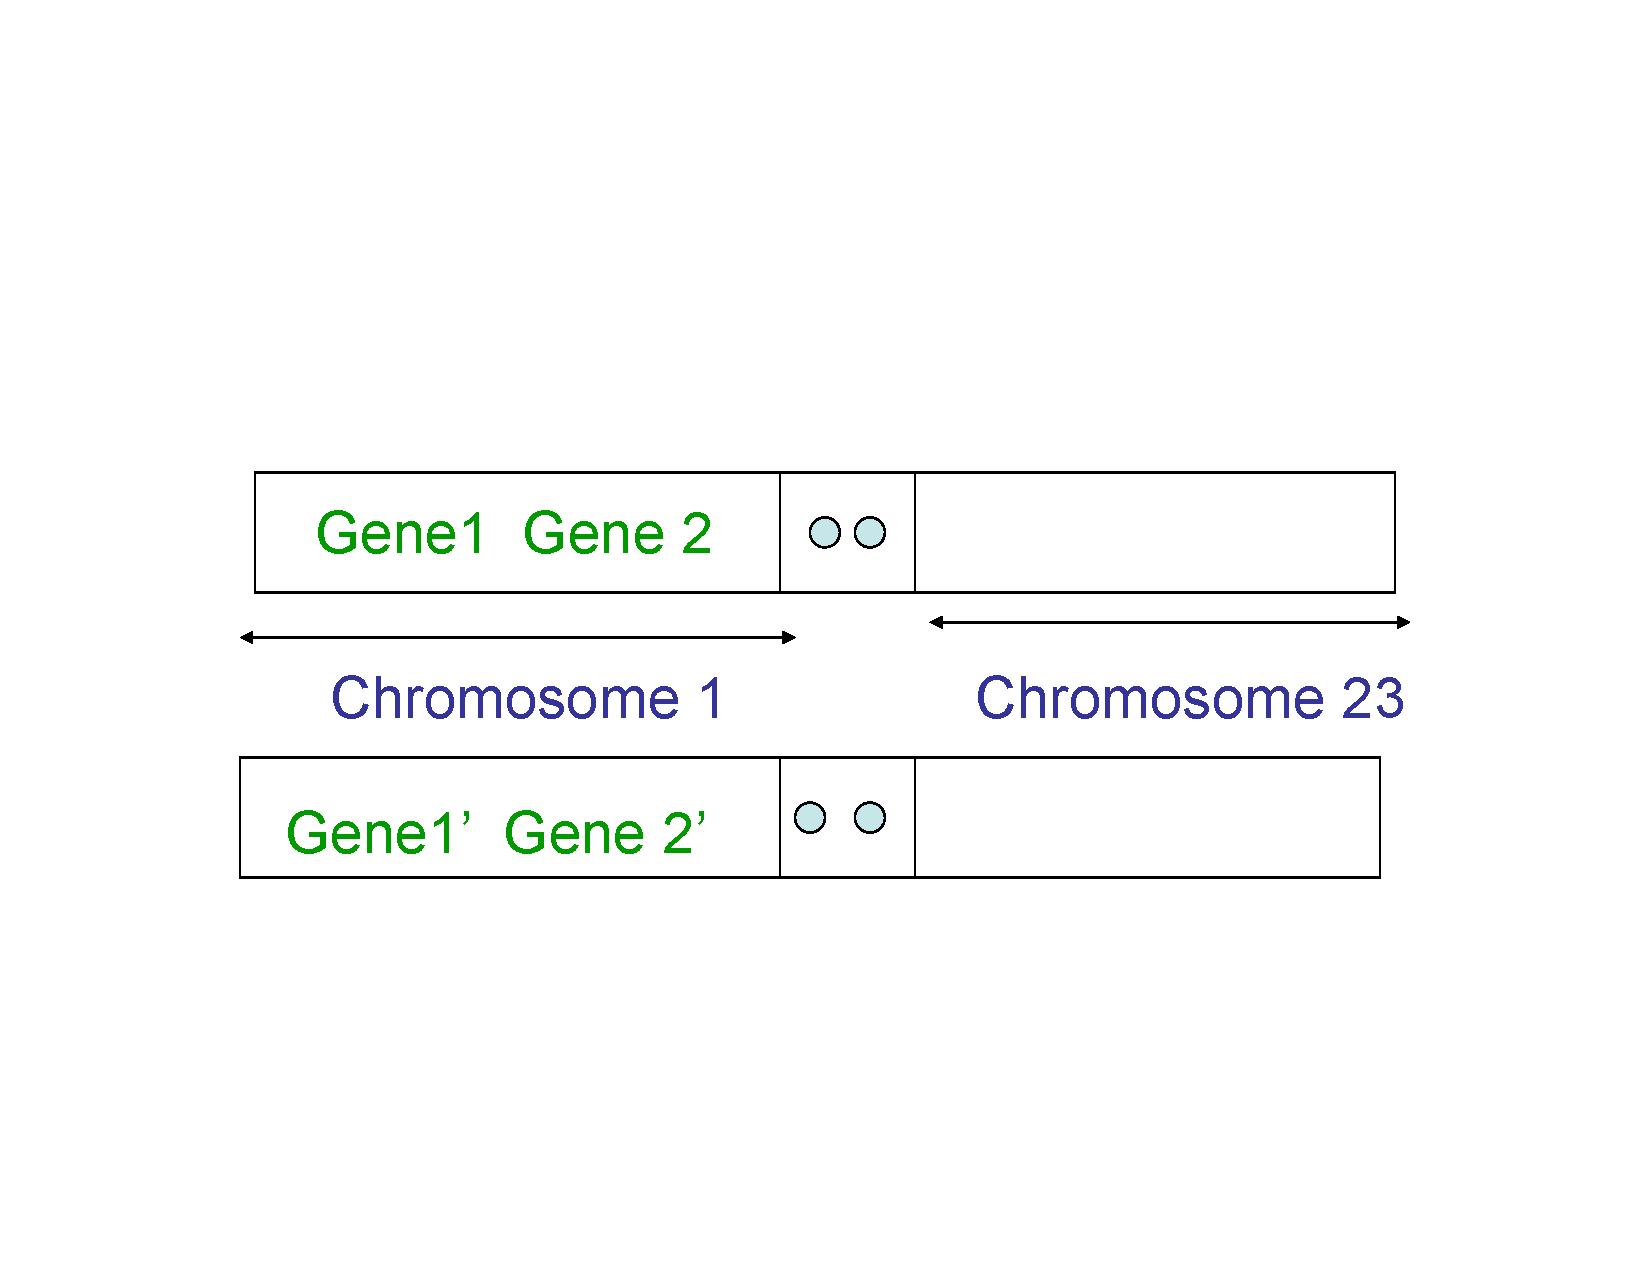
\includegraphics[trim = 0mm 60mm 0mm 80mm, clip, width=4.5in]{fig/chromosomes.pdf}
\caption{A human genotype has two programs modularized into 23
  chromosomes each and in which chromosome contains genes, analogous
  to function blocks in code.}
  \label{fig:chromosomes}
\end{figure}

A first level approximation of how these programs interact is
Mendelian via dominance --- each gene controls one trait (e.g.,
whether one curl one�s tongue) and one of the two functions in each
program exercises control of the function and the other gene is
essentially absent or recessive.  The truth is more complicated: some
functions such as eye color are controlled by both programs, some
traits are controlled by multiple genes in concert, and some genes are
controlled by multiple traits.  Nevertheless, DNA controls traits so
even the simplest queries on DNA are useful, e.g.,

Sample DNA query: Compared to a `standard' patient, are there parts of
the patient's DNA program (especially genes that affect health) that
has been altered?
  
\subsection{Program Composition --- Heredity and Sex}

Many important queries to genetic data are to address about heredity:
for example, is a disease inherited from parents? We provide a simple
model for how parents pass on traits to offspring by passing on
functional blocks (genes) to children.  The fundamental problem is to
take 2 programs, from the father and a different 2 programs from the
mother, and produce 2 new programs for the child in way that maximizes
variety.  This is done in two stages.  In the first stage, each
partner in mating produces a so-called haploid sex cell that has only
one program by a randomized reduction called crossover that is done as
part of a process called meiosis.

A simple functional description of crossover is that for each pair of
homologous chromosomes a new chromosome is formed by splicing together
a random prefix (Fig.~\ref{fig:recombination}) of one chromosome in
the pair with the corresponding suffix of the other chromosome in the
pair.  Thus the egg cell of the mother (and the sperm cell of the
father) has 1 program that is a randomized combination of the
chromosomes the mother (father) inherited from their parents.
Finally, in fertilization, the two sex cells unite to form a zygote
with two programs again, one from each sex cell.  Since each sex cell
and sperm cell form different randomized combinations, each child is
effectively a different randomized mixture of its four grandparents.
Such inheritance of programs suggest the simple query:

  

Figure 4:
\begin{figure}[h!]
  \centering
  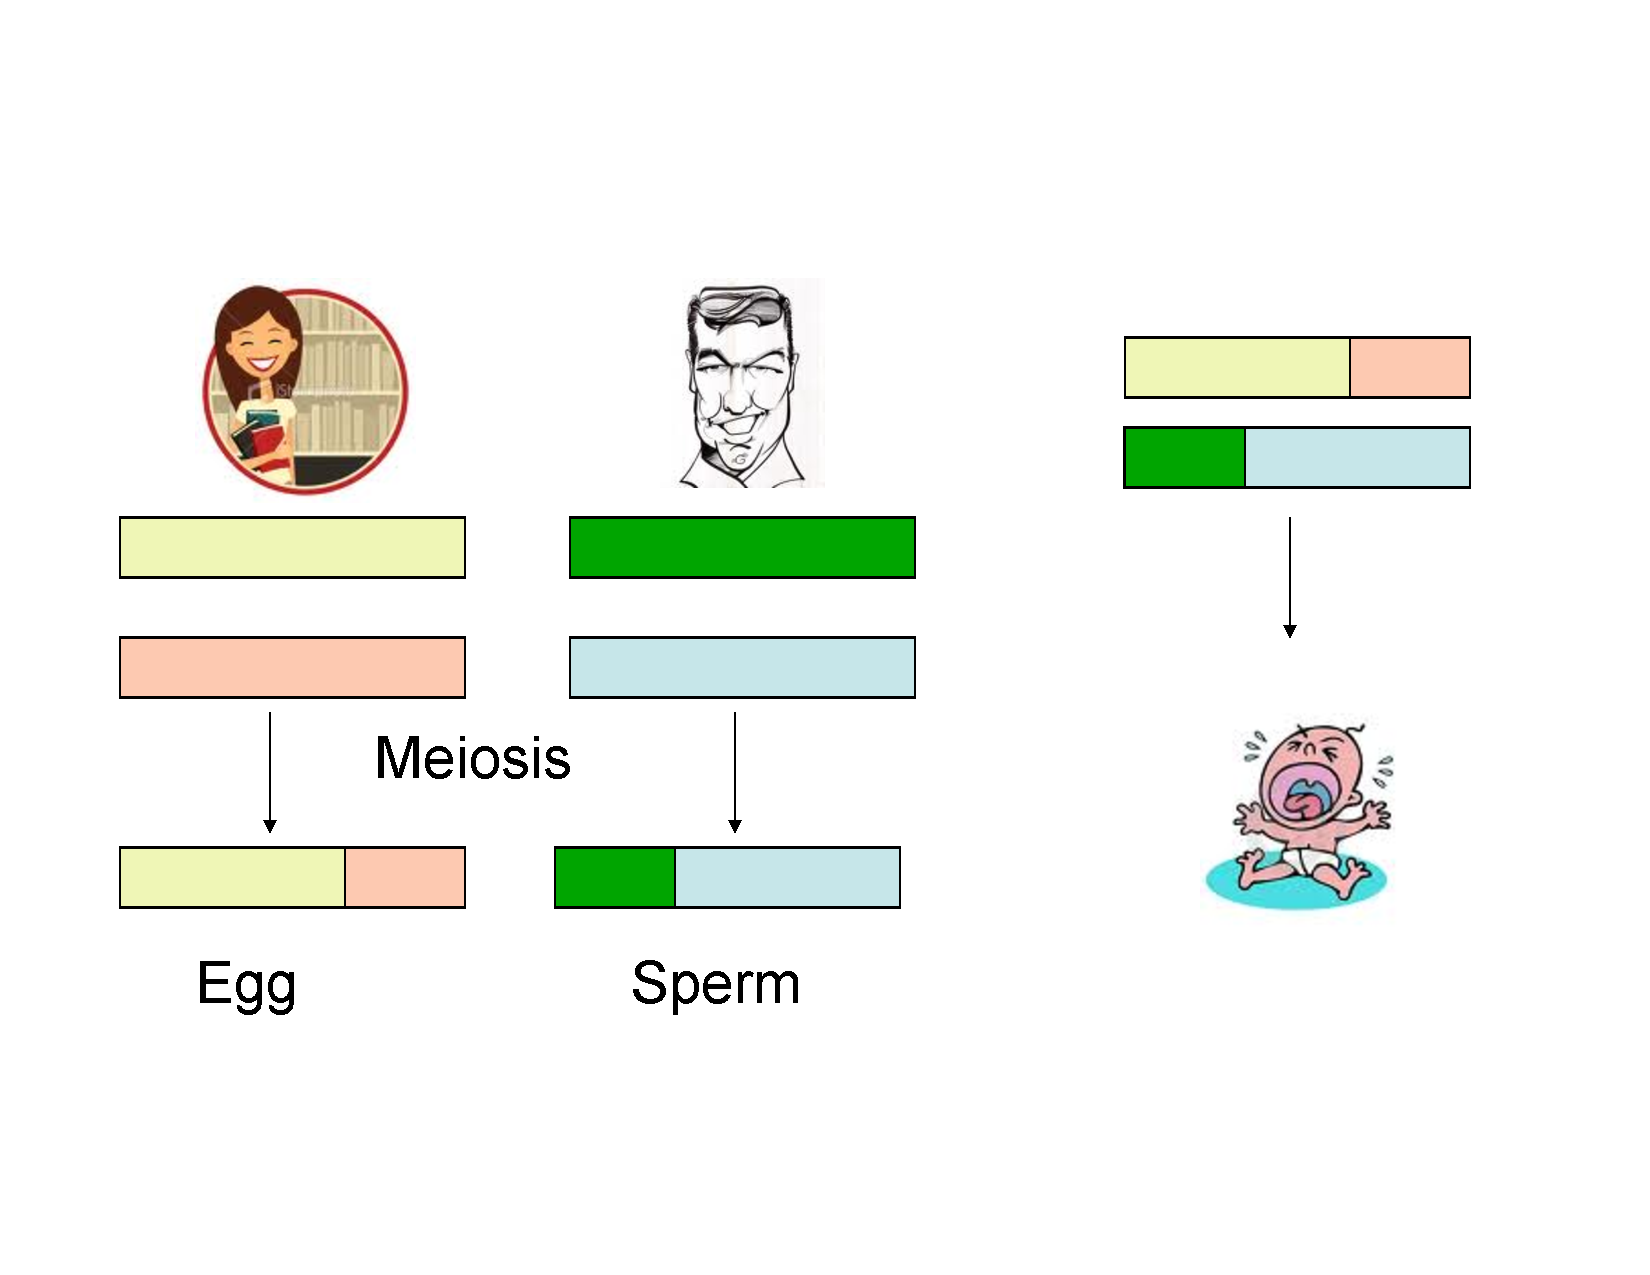
\includegraphics[trim = 10mm 30mm 20mm 40mm, clip, width = 4in]{fig/recombination.pdf}
  \caption{A baby's program is the composition of the programs of the
    mother and father. First, the two programs of each parent are
    `reduced' to a single program in the sex cell by randomized
    splicing.  Next, the two single programs are juxtaposed in the
    baby cell.}
  \label{fig:recombination}
\end{figure}


Sample Inheritance Query: Given a faulty gene, which parent did the
patient receive it from?  What are the chance of the patient passing
it on to his or her children?

The composition is not completely random, however, because of
crossover --- it is more probable that 2 genes are that are closer
together in a parent chromosome will be passed on to a child than 2
genes that are further apart, a phenomemon known as linkage.  There is
more fine print.  For example, one of the 23 chromosomes is called the
sex chromosome and come in two forms X and Y, with males having XY and
females having YY: unlike other chromosomes the X chromosome is
smaller than the Y chromosome and so the simple crossover model does
not apply there.  Further, there can be multiple crossovers where the
sex cell program consists of a prefix and a suffix from 1 chromosome
and middle from the second.  It is best to ignore these complexities
to make progress on abstractions while realizing that the dance of
life is intricate and beautiful.

While a baby starts off as a single cell (gamete), the baby grows by
cell copying (mitosis) as shown in Figure~\ref{fig:differentiation}.
Each copying step ideally copies the program of the parent cell.  The
initial cells are stem cells that can perform any function.  At some
stage, cells specialize to form liver cells, blood cells etc.  Note
that each such cell has the same program as any other cell but
apparently has some additional state that directs only some parts of
the overall program to run (some genes to express).  The copying
process has a number of checks and balances but it is possible for an
erroneous copy to arise which can lead to disease.





%Figure 5:
\begin{figure}[h!]
  \centering
  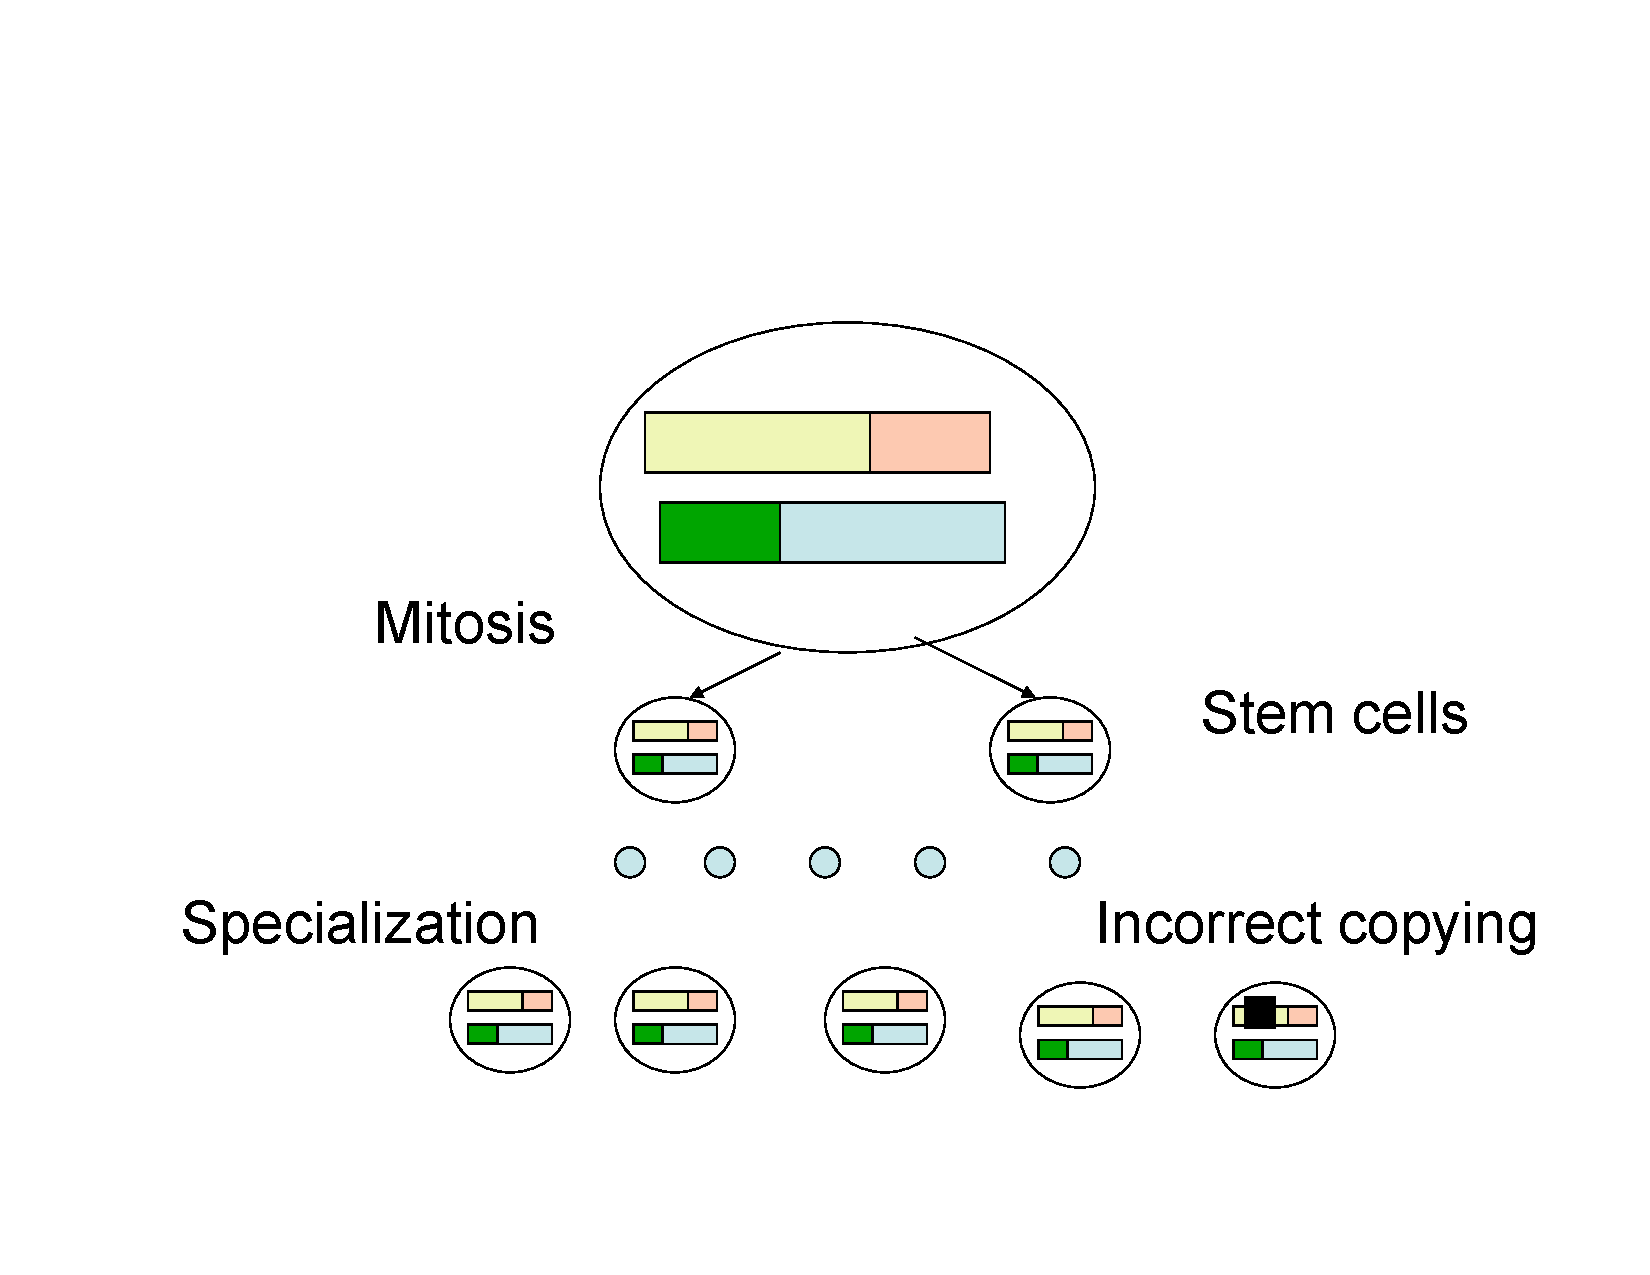
\includegraphics[trim = 0mm 0mm 0mm 0mm, clip, width=4.5in]{fig/differentiation.pdf}
  \caption{The single `zygote' baby cell grows by a copying process
    called mitosis followed by specialization into blood, muscle cells
    etc.  Incorrect copying can also occur.}
  \label{fig:differentiation}
\end{figure}


\subsection{2.3 Run time Microcode: DNA to RNA to Protein}
\label{sec:genes}
 
So far we have examined the DNA program statically.  When a `gene'
runs, the execution path is as follows.  The gene program is stored in
the nucleus of the cell almost like in ROM.  However, execution occurs
in one of many `ribosomes' (analogous to a CPU) .  Information travels
from the nucleus to the ribosome via a `messenger' called mRNA that
makes a copy of the gene called a transcript which then goes to the
ribosome (Figure~\ref{fig:centraldogma}).  The ribosome then
translates this program to a protein as follows.

\begin{figure}[h!]
  \centering
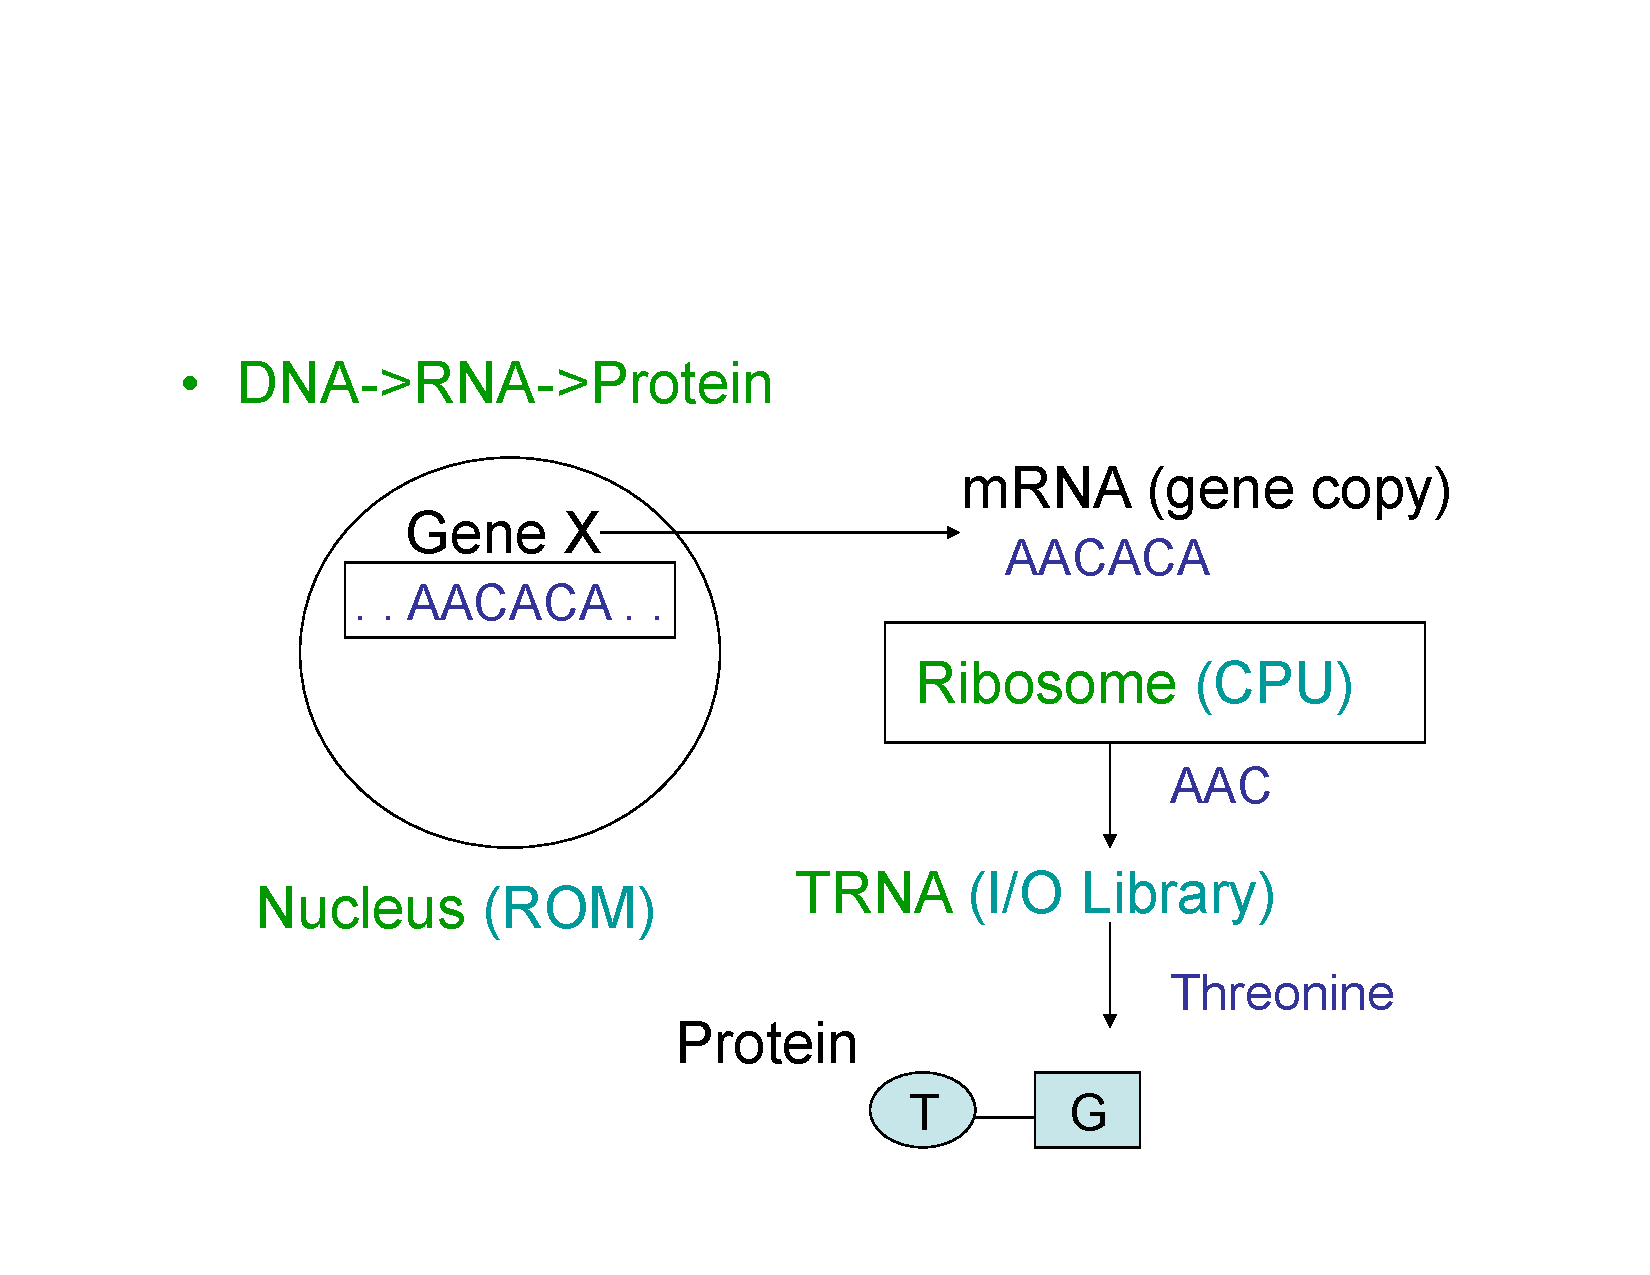
\includegraphics[trim=10mm 10mm 20mm 40mm, clip, width=4.5in]{fig/centraldogma.pdf}  
\caption{A gene program executes by having the instructions fetched by
  mRNA to the ribosome where it is executed by converting each
  3-character opcode (e.g., AAC) into an amino acid (e.g., threonine)
  and concatenating amino acids till a stop codon arrives.}
  \label{fig:centraldogma}
\end{figure}

The ribosome `reads' the gene program 3 bases at a time.  Each 3 base
combination can the thought of an OpCode of an instruction (codon)
that specifies a specific Amino acid. Althought there are $4\times 4\times 4$
combinations of OpCodes, several codons specify the same amino acid:
there are only 20 amino acids, and the mapping from codons to Amino
Acids is called the genetic code.  A protein is the sequence of amino
acids specified the codons in the gene.  The actual assembly of amino
acids into the resulting protein is the function of so-called tRNA
that fetches the specified amino acid and links it to the growing
chain of amino acids.  When the ribosome reaches a special codon
called the Stop codon, the assembly process stops and a protein is
produced.  Proteins are the agents of life: they build cells and help
cells do their specified function.  RNA transcripts are logs of
run-time program activity and can be used for diagnostics.  A sample
RNA query could be:

Sample RNA Query: In a cancerous cell's RNA transcript, which genes
are expressed more than other genes? This may provide insight into the
genes implicated in a cancer.

\subsection{2.4 Higher Level Branching: Operon Model and Pathways}
\label{sec:pathways}
Section~\ref{sec:genes} explained how a `gene' executed and produced a
protein.  However, this was a description of the microcode, so to
speak.  It begs the question as to how the program decides which genes
to execute.  The entire running of the program is shrouded in mystery
but there are some high level patterms that are understood.

First, simple IF-THEN-ELSE branching is often seen in gene execution
via the so-called operon model. As shown in
Figure~\ref{fig:branching}, a group of genes often is controlled by
two entry points called the Repressor and Operon (also a piece of
code).  The figure shows the operon and repressor for two genes that
produce the protein Galactose that helps convert milk into sugar.
When program execution reaches the Repressor, the Repressor produces a
protein that physically joins to the Operon site and blocks the
reading of the program counter beyond the Operon.



\begin{figure}[h!]
  \centering
  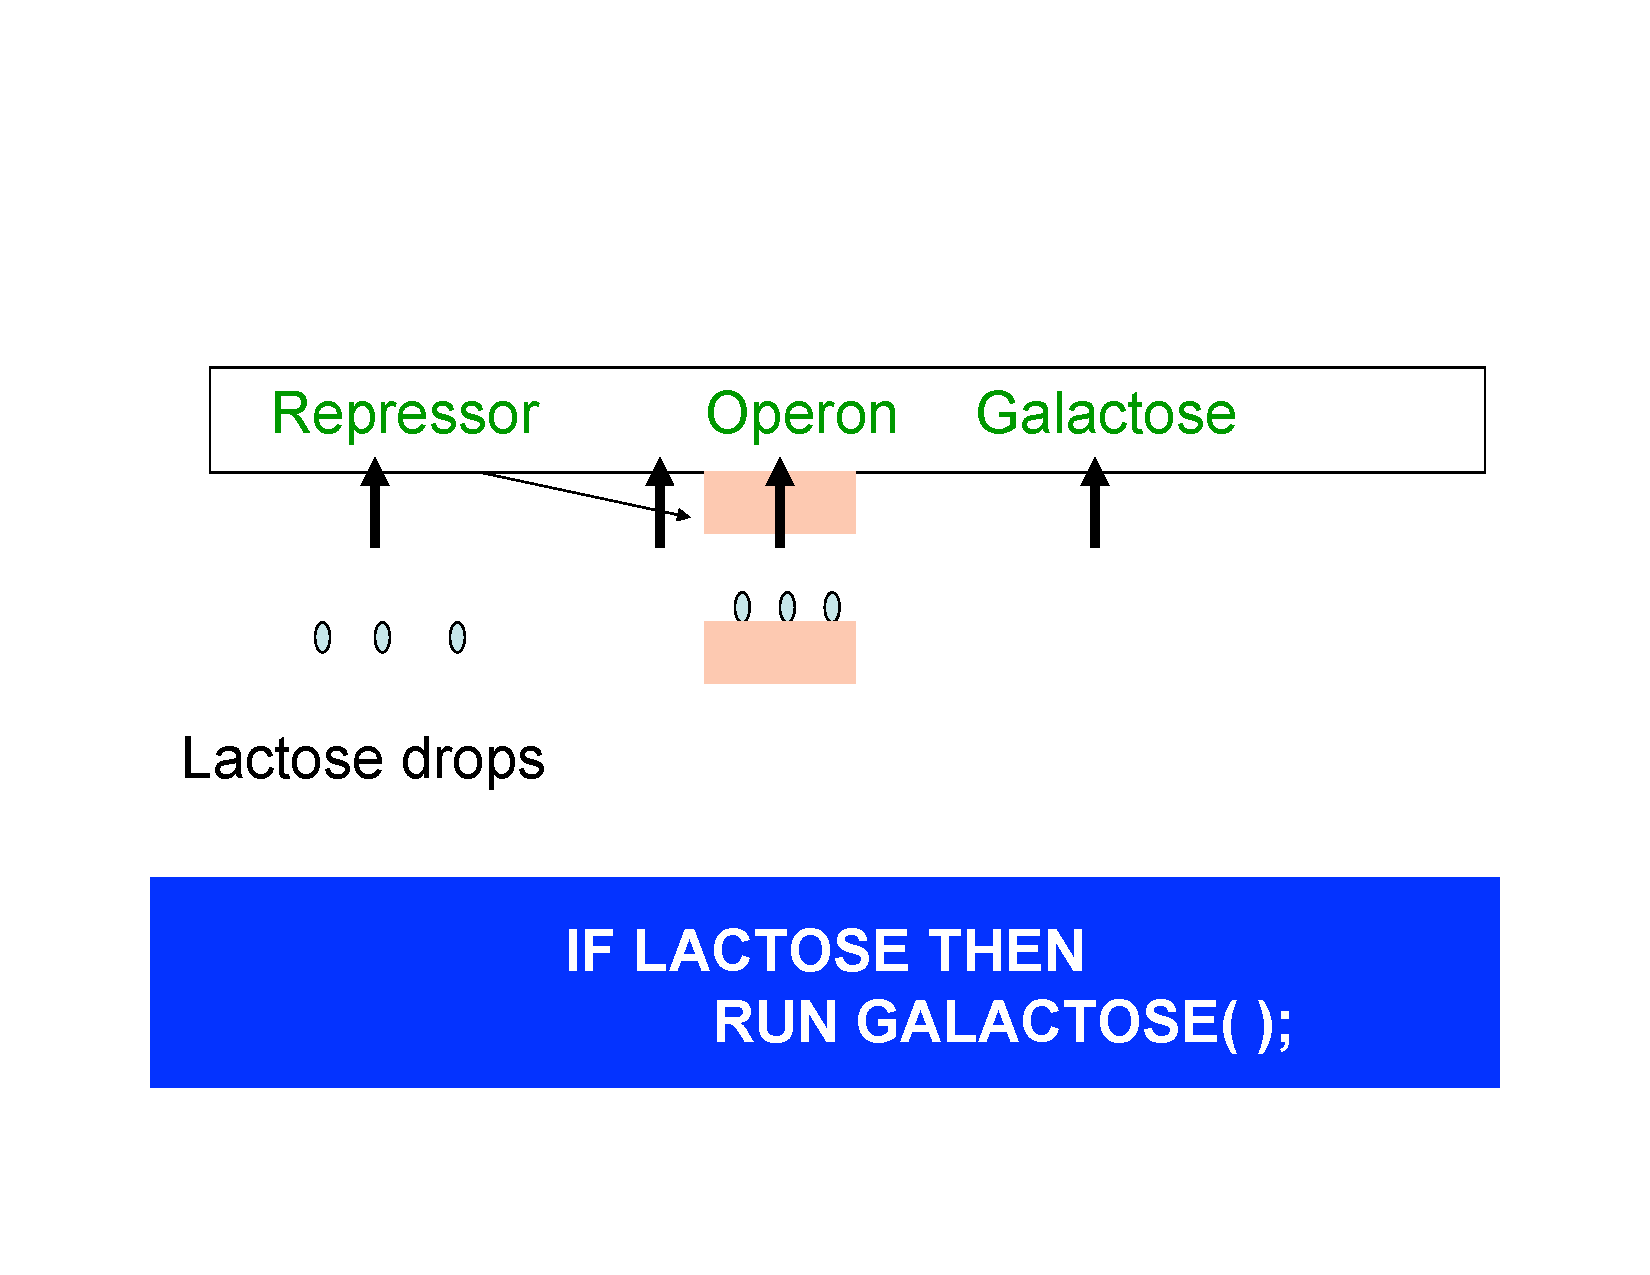
\includegraphics[trim = 20mm 20mm 20mm 30mm, clip, width=4.5in]{fig/branching.pdf}
  \caption{IF-THEN branching via the operon model.  The
    galactose code is run if and only if there are lactose branching.
    Note the physical implementation of branching.}
  \label{fig:branching}
\end{figure}

Thus the Galactose code is not run, and it is not produced.  If milk
or lactose drops enter the cell by digestion, then the lactose binds
with the protein produced by the repressor to form a new substance
that does not bind to the Operon.  This allows the Program counter to
go past the Operon (no longer blocked) and produce Galactose.  From a
computer science perspective, we have:

IF LACTOSE then GALACTOSE(); 

Note that the presence of lactose is an environmental factor, and note
that branching is actually accomplished by physical means such as
binding to an operon site.

Figure~\ref{fig:pathway} shows a more complex branching paradigm
called a pathway which is a generalization of this simple branching.
A pathway can be considered to a be graph in which the nodes are
either genes or enviromental factors and an edge from node A to node B
indicates either that the running of node A will induce the running of
node B or will suppress the running of node B, In our example, the
presence of PolyAcyclic Hydrocarbons {\bf NOTE: Do we have to introduce
the term PAH that \fref{fig:pathway} uses?} in a cell that arise from smoke,
can lead to the `execution' of two genes, that can result downstream
in the production of a bad protein called a carcinogen that produces
cancer.

\begin{figure}[h!]
  \centering
  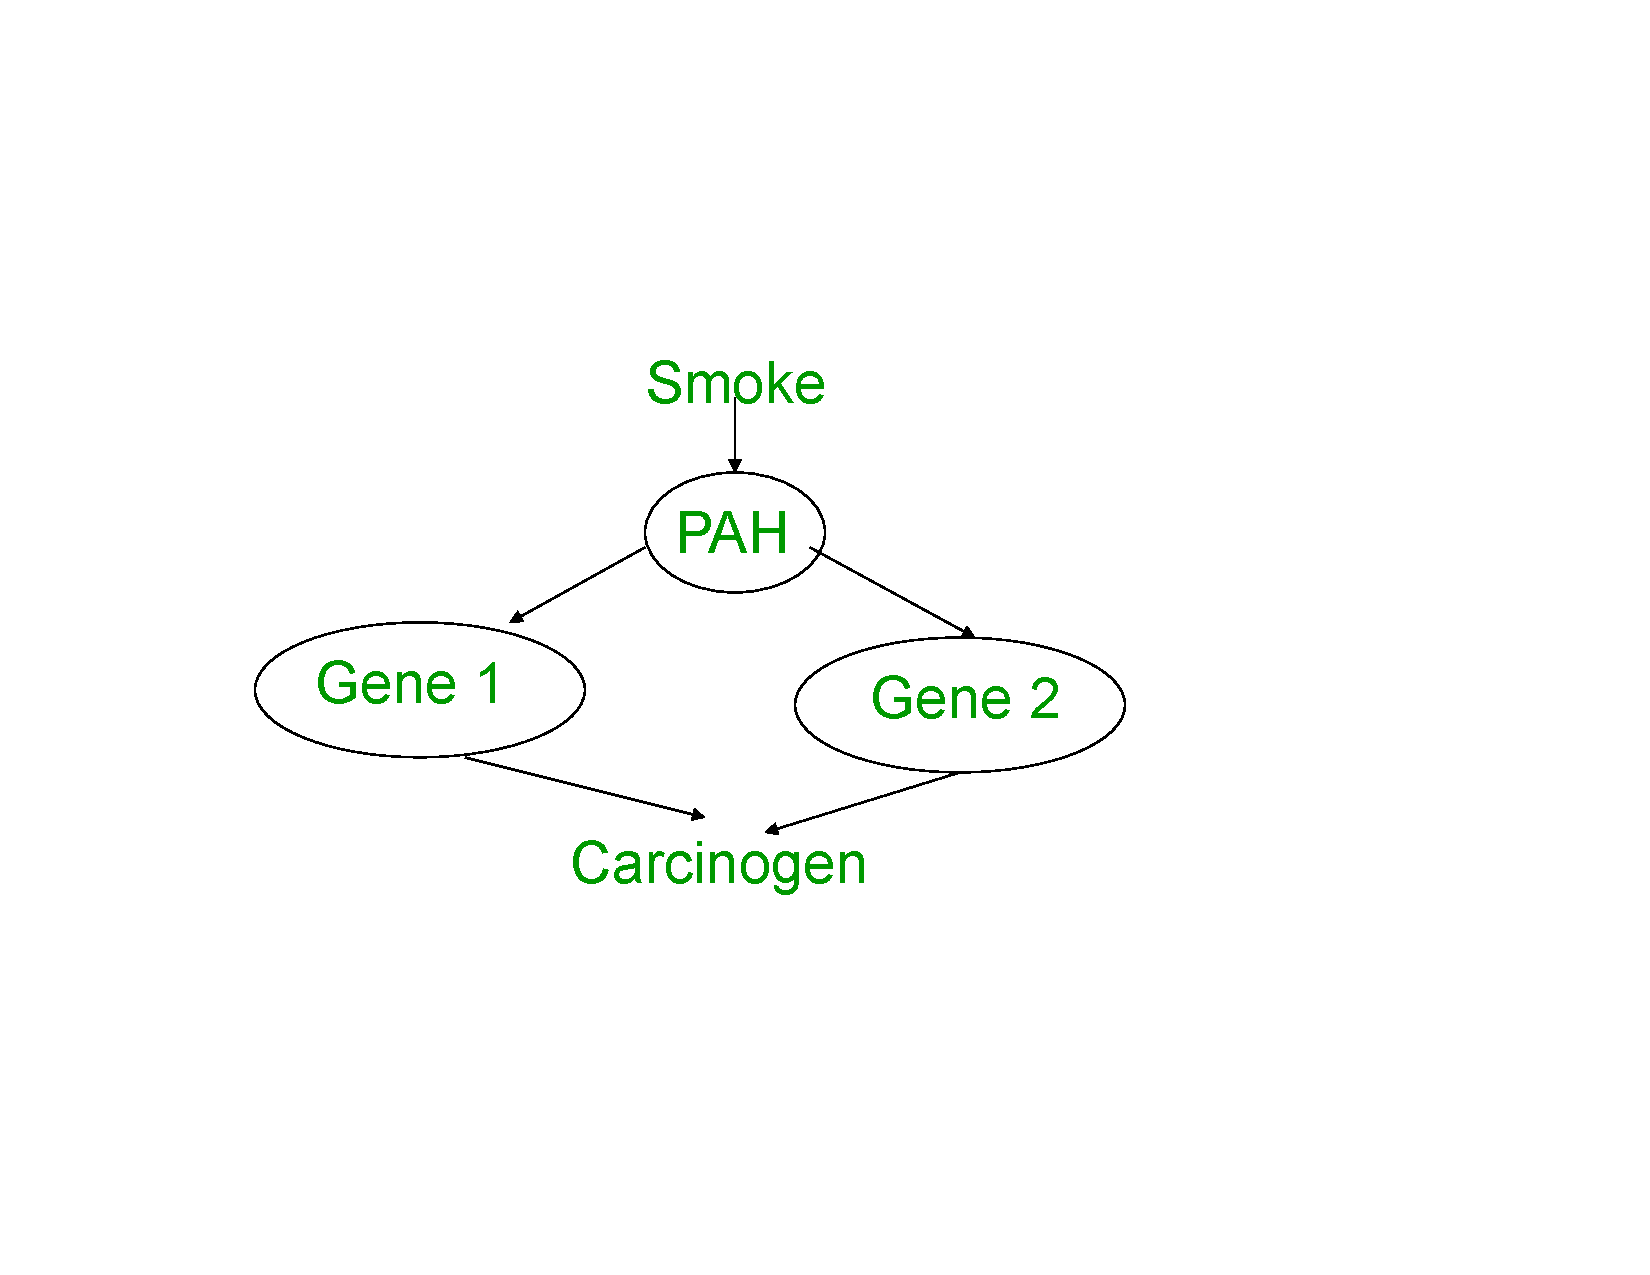
\includegraphics[trim = 40mm 60mm 40mm 40mm, clip, width=4.5in]{fig/pathway.pdf}
  \caption{A more complicated pathway of `influence' where
    physical substances (e.g., smoke) induce genes which then induce
    other genes.  The pathway is represented as a directed acyclic
    graph with directed edges representing influence.}
  \label{fig:pathway}
\end{figure}


Pathways are of great interest to drug designers, physicians, and
biologists.  For example, to prevent cigarette smoking from causing
cancer, it may suffice to interfere with some node in the pathway, for
example by a drug that represses the production of Gene 1.  This leads
to the sample query

Sample Pathway Query: In an RNA transcript of a new disease, is some
existing pathway for some other disease activated (hence can we reuse
older drugs for the new disease)?

\subsection{2.5 Program Analysis Tools: Microarrays and High Throughput Sequencing}
\label{sec:analysistools}
It is only recently that scientists have succeeded in reading the DNA
programs of human beings, The first method that is quite mature is via
DNA microarrays, and the second is called High Throughput Shotgun
sequencing.  Each method has its imperfections and it is important for
the computer scientists to understand their limitations abstractly so
that they see why even simple queries require a great deal of
inference to answer with confidence.

DNA microrrays- Content Based Sampling: Microarrays provide a way to
sample a given DNA sample at some specific locations.  Unlike memory
technology, where we can index into a position, `sampling' is done via
content.  Imagine the sample program was AUGAAGUAG.  Suppose the first
five common to most humans, but the 6th location is a variation called
a SNP (single character variation) in which most of the population has
a G but a few have a U and that is indicative of a disease.  To check
whether the given human being has an A, we cannot read the 6-th
position, but we can ask whether the substring AUGAAU is contained in
the program.  In effect, we are guessing the 6th position and adding
some flanking (and possibly trailing content) that disambiguates the
position.  In practice, a DNA microarray is an array of say 100,000
such queries and the DNA sample is passed over all these queries in
parallel.  Thus a single cell manufactured by hardware vendors such as
Affymetrix or Illumina can identify 100,000 SNPs in a single run at
low cost (around a \$100 in volume).

High-throughput Shotgun Sequencing: Microarrays are good if there is a
limited amount of variation and one knows in advance what possible
variations might exist (for example, a SNP of either a G or a U in a
position).  But when there is massive variaition in the genome, such
sampling simply does not scale.  Instead, current technology has found
a cheap (but imperfect) way to read the genome called shotgun
sequencing.  The idea is shown in Figure~\ref{fig:NGS}.{\bf NOTE:
shotgun sequencing??? This sounds like first generation sequencing
right?}

\begin{figure}[h!]
  \centering
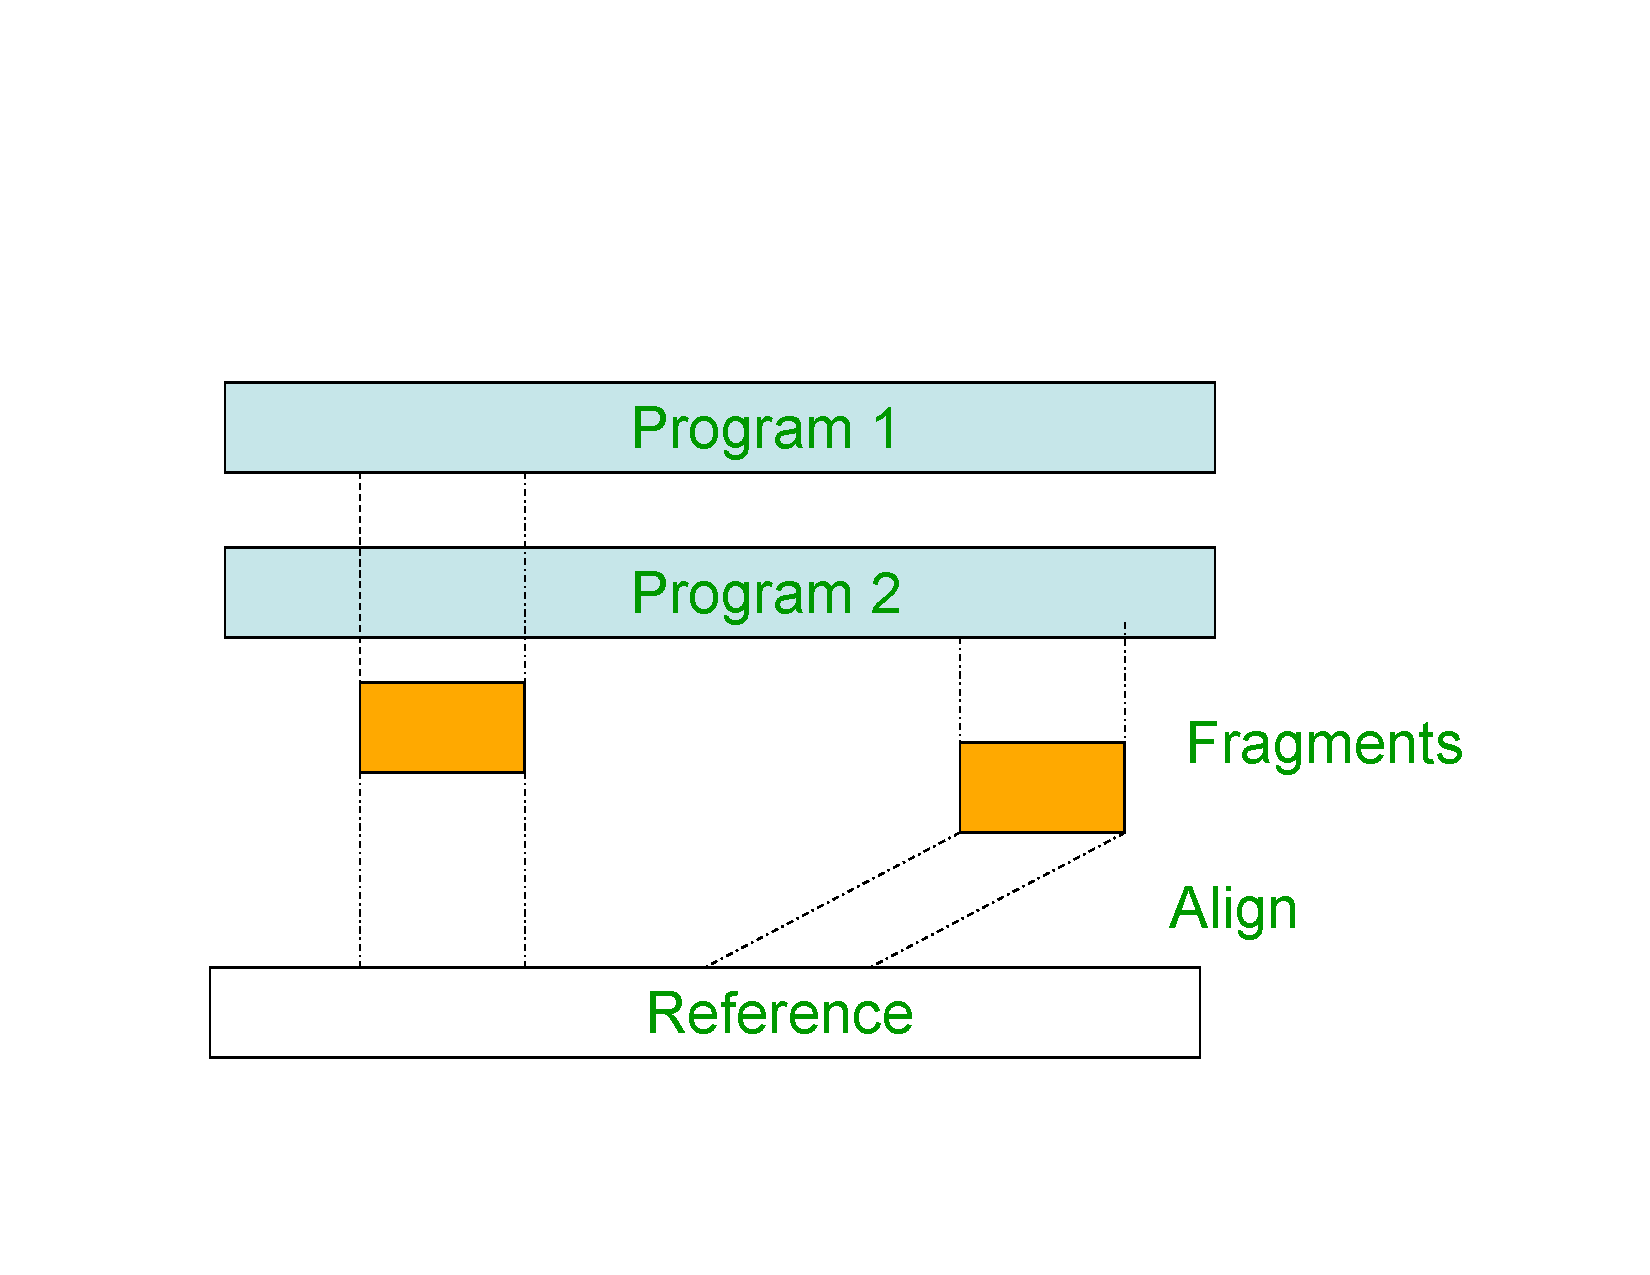
\includegraphics[trim = 10mm 10mm 10mm 30mm, clip, width=4in]{fig/ngs.pdf}  
  \caption{In high-throughput sequencing, the 2 programs fragments are
    randomly selected from either program and enough fragments are
    taken to make it likely that the entire length of the program
    (genome) is `covered'.  Finally, instead of assembling the
    fragments, they are aligned or mapped to matching positions in a
    reference program.}
  \label{fig:NGS}
\end{figure}

First, a physical process is used to randomly cut the DNA program of
the patient sample into small pieces called fragments of small length
L (100 base pairs in older technology to 10,000 in recent ones).{\bf
NOTE: WHAT??? 100bp in newer technology, 10K in older ones}  Each
fragment can be considered to be generated by picking one of the two
programs (from mother or father) at random, picking a random offset
with uniform probability from 1 to the length of the program, and then
selecting the L length string that starts at that offset.  This can be
done by many physical means including sonication via sound waves.
Next, each fragment is actually read in terms of the sequence of bases
in each fragment.

There are a number of technologies for Reading (see appendix) but it
suffices to say that Reads cannot proceed reliably beyond a certain
length.  Hence, the current approach is to break up the long DNA into
bite-sized random fragments that are small enough to be read.
Enough fragments are created such that if they were lined up, the
total length of the fragments would be some multiple (called the
coverage, factors of 10 are available today) of the length of the
genome being sequenced.

While the natural assumption is that these fragments will be assembled
like a giant jigsaw puzzle, this turns out to be complex and expensive
because of the large amounts of repetitive portions in human genomes
that create aliasing effects that are hard to disambiguate. {\bf NOTE: A non
knowledgable audience might need pointers that describe the problems
of the assembly} Instead,
the fragments are aligned or mapped to a so-called reference human
genome.  Mapping simply means finding a substring on the reference
genome that matches the characters in the fragment up to a small
number of errors.  In case of multiple matches, the `best' match is
returned, sometimes with some alternatives.

The human reference genome, oddly enough, is a single (haploid)
program.  It was found at great expense by the celebrated human genome
project and reflects a composite reference formed out of several
individuals including Craig Venter.  Again, owing to the complexities
of complete assembly, it reflects a political consensus on what a
reference should be.  Mapping new patient genomes works because string
search is cheaper than assembly and because most human genomes
(including the 2 programs in each human) are 99\% similar.  Thus,
while a 2-program (diploid) reference may have been ideal, the current
reference is 1-program.  It is often augmented with a list of common
variations (SNPs) called SNPdb.
{\bf NOTE: I don't see the point of this paragraph. Why is it a
political consensus on what a reference should be? Also what is the
point of the last sentence?}

\newpage
\section{The Formal Grammar}
\begin{grammar}
      [(colon){$\rightarrow$}]
      [(semicolon)$|$]
      [(comma){}]
      [(period){\\}]
      [(quote){\begin{bf}}{\end{bf}}]
      [(nonterminal){$\langle$}{$\rangle$}]
<program>: <table\_prototypes> <assigned\_selects>
<select\_statement>.
<table\_prototypes>: <table\_prototype>
<table\_prototypes>;"$\epsilon$".
<table\_prototype>: <table\_keyword> "(" table\_args ")" ";".
<table\_keyword>: "TABLE" <names>.
<names>: "ID".
<table\_args>: <table\_arg> "," <table\_args> ; <table\_arg>.
<table\_arg>: "INTEGER" <names>; "FLOAT" <names>; "CHAR" <names>;
"STRING" <names>.
<assigned\_selects>: <assigned\_select> <assigned\_selects>;"$\epsilon$".
<assigned\_select>: <lvalue> "=" <select\_statement>.
<l\_value>: <names>.
<select\_statement>: "SELECT" <select\_args> "FROM" <from\_args>
"WHERE" <where\_args>.
<select\_args>: "*"; "COUNTVECTOR"; <select\_arg\_series>.
<select\_arg\_series>: <names> "," <select\_arg\_series>; <names>.
<from\_args>: <from\_arg> "," <from\_args>; <from\_arg>.
<from\_arg>: <names>.
<where\_args>: <where\_args> "," <where\_args>;
<where\_args> "AND" <where\_args>;<where\_args> "OR" <where\_args>;
"NOT" where\_args;"(" where\_args ")";<lowest\_expr>.
<lowest\_expr>: <arith\_expr> <comparison\_op> <rvalue>.
<arith\_expr>: <arith\_expr> <arith\_op> <arith\_expr>;
<arith\_op> <arith\_expr>;
<names>;
<number>.
<comparison\_op>: "$==$"; "$>=$"; "$>$"; "$<=$"; "$<$".
<arith\_op>: "+"; "-";"*";"/"; "\%".
<rvalue>: <const\_char>; <const\_str>; <number>.
<const\_char>:"`" "[A-Z][a-z]" "'".
<const\_str>: "``" <names> "''".
<number>: <digit> <number>; <digit>.
<digit>:"0";"1";"2";"3";"4";"5";"6";"7";"8";"9".

\end{grammar}


\end{document}


